\documentclass[11pt]{article}

    \usepackage[breakable]{tcolorbox}
    \usepackage{parskip} % Stop auto-indenting (to mimic markdown behaviour)
    
    \usepackage{iftex}
    \ifPDFTeX
        \usepackage[T1]{fontenc}
        \usepackage{mathpazo}
    \else
        \usepackage{fontspec}
    \fi

    % Basic figure setup, for now with no caption control since it's done
    % automatically by Pandoc (which extracts ![](path) syntax from Markdown).
    \usepackage{graphicx}
    % Maintain compatibility with old templates. Remove in nbconvert 6.0
    \let\Oldincludegraphics\includegraphics
    % Ensure that by default, figures have no caption (until we provide a
    % proper Figure object with a Caption API and a way to capture that
    % in the conversion process - todo).
    \usepackage{caption}
    \DeclareCaptionFormat{nocaption}{}
    \captionsetup{format=nocaption,aboveskip=0pt,belowskip=0pt}

    \usepackage[Export]{adjustbox} % Used to constrain images to a maximum size
    \adjustboxset{max size={0.9\linewidth}{0.9\paperheight}}
    \usepackage{float}
    \floatplacement{figure}{H} % forces figures to be placed at the correct location
    \usepackage{xcolor} % Allow colors to be defined
    \usepackage{enumerate} % Needed for markdown enumerations to work
    \usepackage{geometry} % Used to adjust the document margins
    \usepackage{amsmath} % Equations
    \usepackage{amssymb} % Equations
    \usepackage{textcomp} % defines textquotesingle
    % Hack from http://tex.stackexchange.com/a/47451/13684:
    \AtBeginDocument{%
        \def\PYZsq{\textquotesingle}% Upright quotes in Pygmentized code
    }
    \usepackage{upquote} % Upright quotes for verbatim code
    \usepackage{eurosym} % defines \euro
    \usepackage[mathletters]{ucs} % Extended unicode (utf-8) support
    \usepackage{fancyvrb} % verbatim replacement that allows latex
    \usepackage{grffile} % extends the file name processing of package graphics 
                         % to support a larger range
    \makeatletter % fix for grffile with XeLaTeX
    \def\Gread@@xetex#1{%
      \IfFileExists{"\Gin@base".bb}%
      {\Gread@eps{\Gin@base.bb}}%
      {\Gread@@xetex@aux#1}%
    }
    \makeatother

    % The hyperref package gives us a pdf with properly built
    % internal navigation ('pdf bookmarks' for the table of contents,
    % internal cross-reference links, web links for URLs, etc.)
    \usepackage{hyperref}
    % The default LaTeX title has an obnoxious amount of whitespace. By default,
    % titling removes some of it. It also provides customization options.
    \usepackage{titling}
    \usepackage{longtable} % longtable support required by pandoc >1.10
    \usepackage{booktabs}  % table support for pandoc > 1.12.2
    \usepackage[inline]{enumitem} % IRkernel/repr support (it uses the enumerate* environment)
    \usepackage[normalem]{ulem} % ulem is needed to support strikethroughs (\sout)
                                % normalem makes italics be italics, not underlines
    \usepackage{mathrsfs}
    

    
    % Colors for the hyperref package
    \definecolor{urlcolor}{rgb}{0,.145,.698}
    \definecolor{linkcolor}{rgb}{.71,0.21,0.01}
    \definecolor{citecolor}{rgb}{.12,.54,.11}

    % ANSI colors
    \definecolor{ansi-black}{HTML}{3E424D}
    \definecolor{ansi-black-intense}{HTML}{282C36}
    \definecolor{ansi-red}{HTML}{E75C58}
    \definecolor{ansi-red-intense}{HTML}{B22B31}
    \definecolor{ansi-green}{HTML}{00A250}
    \definecolor{ansi-green-intense}{HTML}{007427}
    \definecolor{ansi-yellow}{HTML}{DDB62B}
    \definecolor{ansi-yellow-intense}{HTML}{B27D12}
    \definecolor{ansi-blue}{HTML}{208FFB}
    \definecolor{ansi-blue-intense}{HTML}{0065CA}
    \definecolor{ansi-magenta}{HTML}{D160C4}
    \definecolor{ansi-magenta-intense}{HTML}{A03196}
    \definecolor{ansi-cyan}{HTML}{60C6C8}
    \definecolor{ansi-cyan-intense}{HTML}{258F8F}
    \definecolor{ansi-white}{HTML}{C5C1B4}
    \definecolor{ansi-white-intense}{HTML}{A1A6B2}
    \definecolor{ansi-default-inverse-fg}{HTML}{FFFFFF}
    \definecolor{ansi-default-inverse-bg}{HTML}{000000}

    % commands and environments needed by pandoc snippets
    % extracted from the output of `pandoc -s`
    \providecommand{\tightlist}{%
      \setlength{\itemsep}{0pt}\setlength{\parskip}{0pt}}
    \DefineVerbatimEnvironment{Highlighting}{Verbatim}{commandchars=\\\{\}}
    % Add ',fontsize=\small' for more characters per line
    \newenvironment{Shaded}{}{}
    \newcommand{\KeywordTok}[1]{\textcolor[rgb]{0.00,0.44,0.13}{\textbf{{#1}}}}
    \newcommand{\DataTypeTok}[1]{\textcolor[rgb]{0.56,0.13,0.00}{{#1}}}
    \newcommand{\DecValTok}[1]{\textcolor[rgb]{0.25,0.63,0.44}{{#1}}}
    \newcommand{\BaseNTok}[1]{\textcolor[rgb]{0.25,0.63,0.44}{{#1}}}
    \newcommand{\FloatTok}[1]{\textcolor[rgb]{0.25,0.63,0.44}{{#1}}}
    \newcommand{\CharTok}[1]{\textcolor[rgb]{0.25,0.44,0.63}{{#1}}}
    \newcommand{\StringTok}[1]{\textcolor[rgb]{0.25,0.44,0.63}{{#1}}}
    \newcommand{\CommentTok}[1]{\textcolor[rgb]{0.38,0.63,0.69}{\textit{{#1}}}}
    \newcommand{\OtherTok}[1]{\textcolor[rgb]{0.00,0.44,0.13}{{#1}}}
    \newcommand{\AlertTok}[1]{\textcolor[rgb]{1.00,0.00,0.00}{\textbf{{#1}}}}
    \newcommand{\FunctionTok}[1]{\textcolor[rgb]{0.02,0.16,0.49}{{#1}}}
    \newcommand{\RegionMarkerTok}[1]{{#1}}
    \newcommand{\ErrorTok}[1]{\textcolor[rgb]{1.00,0.00,0.00}{\textbf{{#1}}}}
    \newcommand{\NormalTok}[1]{{#1}}
    
    % Additional commands for more recent versions of Pandoc
    \newcommand{\ConstantTok}[1]{\textcolor[rgb]{0.53,0.00,0.00}{{#1}}}
    \newcommand{\SpecialCharTok}[1]{\textcolor[rgb]{0.25,0.44,0.63}{{#1}}}
    \newcommand{\VerbatimStringTok}[1]{\textcolor[rgb]{0.25,0.44,0.63}{{#1}}}
    \newcommand{\SpecialStringTok}[1]{\textcolor[rgb]{0.73,0.40,0.53}{{#1}}}
    \newcommand{\ImportTok}[1]{{#1}}
    \newcommand{\DocumentationTok}[1]{\textcolor[rgb]{0.73,0.13,0.13}{\textit{{#1}}}}
    \newcommand{\AnnotationTok}[1]{\textcolor[rgb]{0.38,0.63,0.69}{\textbf{\textit{{#1}}}}}
    \newcommand{\CommentVarTok}[1]{\textcolor[rgb]{0.38,0.63,0.69}{\textbf{\textit{{#1}}}}}
    \newcommand{\VariableTok}[1]{\textcolor[rgb]{0.10,0.09,0.49}{{#1}}}
    \newcommand{\ControlFlowTok}[1]{\textcolor[rgb]{0.00,0.44,0.13}{\textbf{{#1}}}}
    \newcommand{\OperatorTok}[1]{\textcolor[rgb]{0.40,0.40,0.40}{{#1}}}
    \newcommand{\BuiltInTok}[1]{{#1}}
    \newcommand{\ExtensionTok}[1]{{#1}}
    \newcommand{\PreprocessorTok}[1]{\textcolor[rgb]{0.74,0.48,0.00}{{#1}}}
    \newcommand{\AttributeTok}[1]{\textcolor[rgb]{0.49,0.56,0.16}{{#1}}}
    \newcommand{\InformationTok}[1]{\textcolor[rgb]{0.38,0.63,0.69}{\textbf{\textit{{#1}}}}}
    \newcommand{\WarningTok}[1]{\textcolor[rgb]{0.38,0.63,0.69}{\textbf{\textit{{#1}}}}}
    
    
    % Define a nice break command that doesn't care if a line doesn't already
    % exist.
    \def\br{\hspace*{\fill} \\* }
    % Math Jax compatibility definitions
    \def\gt{>}
    \def\lt{<}
    \let\Oldtex\TeX
    \let\Oldlatex\LaTeX
    \renewcommand{\TeX}{\textrm{\Oldtex}}
    \renewcommand{\LaTeX}{\textrm{\Oldlatex}}
    % Document parameters
    % Document title
    \title{Ausarbeitung}
    
    
    
    
    
% Pygments definitions
\makeatletter
\def\PY@reset{\let\PY@it=\relax \let\PY@bf=\relax%
    \let\PY@ul=\relax \let\PY@tc=\relax%
    \let\PY@bc=\relax \let\PY@ff=\relax}
\def\PY@tok#1{\csname PY@tok@#1\endcsname}
\def\PY@toks#1+{\ifx\relax#1\empty\else%
    \PY@tok{#1}\expandafter\PY@toks\fi}
\def\PY@do#1{\PY@bc{\PY@tc{\PY@ul{%
    \PY@it{\PY@bf{\PY@ff{#1}}}}}}}
\def\PY#1#2{\PY@reset\PY@toks#1+\relax+\PY@do{#2}}

\expandafter\def\csname PY@tok@w\endcsname{\def\PY@tc##1{\textcolor[rgb]{0.73,0.73,0.73}{##1}}}
\expandafter\def\csname PY@tok@c\endcsname{\let\PY@it=\textit\def\PY@tc##1{\textcolor[rgb]{0.25,0.50,0.50}{##1}}}
\expandafter\def\csname PY@tok@cp\endcsname{\def\PY@tc##1{\textcolor[rgb]{0.74,0.48,0.00}{##1}}}
\expandafter\def\csname PY@tok@k\endcsname{\let\PY@bf=\textbf\def\PY@tc##1{\textcolor[rgb]{0.00,0.50,0.00}{##1}}}
\expandafter\def\csname PY@tok@kp\endcsname{\def\PY@tc##1{\textcolor[rgb]{0.00,0.50,0.00}{##1}}}
\expandafter\def\csname PY@tok@kt\endcsname{\def\PY@tc##1{\textcolor[rgb]{0.69,0.00,0.25}{##1}}}
\expandafter\def\csname PY@tok@o\endcsname{\def\PY@tc##1{\textcolor[rgb]{0.40,0.40,0.40}{##1}}}
\expandafter\def\csname PY@tok@ow\endcsname{\let\PY@bf=\textbf\def\PY@tc##1{\textcolor[rgb]{0.67,0.13,1.00}{##1}}}
\expandafter\def\csname PY@tok@nb\endcsname{\def\PY@tc##1{\textcolor[rgb]{0.00,0.50,0.00}{##1}}}
\expandafter\def\csname PY@tok@nf\endcsname{\def\PY@tc##1{\textcolor[rgb]{0.00,0.00,1.00}{##1}}}
\expandafter\def\csname PY@tok@nc\endcsname{\let\PY@bf=\textbf\def\PY@tc##1{\textcolor[rgb]{0.00,0.00,1.00}{##1}}}
\expandafter\def\csname PY@tok@nn\endcsname{\let\PY@bf=\textbf\def\PY@tc##1{\textcolor[rgb]{0.00,0.00,1.00}{##1}}}
\expandafter\def\csname PY@tok@ne\endcsname{\let\PY@bf=\textbf\def\PY@tc##1{\textcolor[rgb]{0.82,0.25,0.23}{##1}}}
\expandafter\def\csname PY@tok@nv\endcsname{\def\PY@tc##1{\textcolor[rgb]{0.10,0.09,0.49}{##1}}}
\expandafter\def\csname PY@tok@no\endcsname{\def\PY@tc##1{\textcolor[rgb]{0.53,0.00,0.00}{##1}}}
\expandafter\def\csname PY@tok@nl\endcsname{\def\PY@tc##1{\textcolor[rgb]{0.63,0.63,0.00}{##1}}}
\expandafter\def\csname PY@tok@ni\endcsname{\let\PY@bf=\textbf\def\PY@tc##1{\textcolor[rgb]{0.60,0.60,0.60}{##1}}}
\expandafter\def\csname PY@tok@na\endcsname{\def\PY@tc##1{\textcolor[rgb]{0.49,0.56,0.16}{##1}}}
\expandafter\def\csname PY@tok@nt\endcsname{\let\PY@bf=\textbf\def\PY@tc##1{\textcolor[rgb]{0.00,0.50,0.00}{##1}}}
\expandafter\def\csname PY@tok@nd\endcsname{\def\PY@tc##1{\textcolor[rgb]{0.67,0.13,1.00}{##1}}}
\expandafter\def\csname PY@tok@s\endcsname{\def\PY@tc##1{\textcolor[rgb]{0.73,0.13,0.13}{##1}}}
\expandafter\def\csname PY@tok@sd\endcsname{\let\PY@it=\textit\def\PY@tc##1{\textcolor[rgb]{0.73,0.13,0.13}{##1}}}
\expandafter\def\csname PY@tok@si\endcsname{\let\PY@bf=\textbf\def\PY@tc##1{\textcolor[rgb]{0.73,0.40,0.53}{##1}}}
\expandafter\def\csname PY@tok@se\endcsname{\let\PY@bf=\textbf\def\PY@tc##1{\textcolor[rgb]{0.73,0.40,0.13}{##1}}}
\expandafter\def\csname PY@tok@sr\endcsname{\def\PY@tc##1{\textcolor[rgb]{0.73,0.40,0.53}{##1}}}
\expandafter\def\csname PY@tok@ss\endcsname{\def\PY@tc##1{\textcolor[rgb]{0.10,0.09,0.49}{##1}}}
\expandafter\def\csname PY@tok@sx\endcsname{\def\PY@tc##1{\textcolor[rgb]{0.00,0.50,0.00}{##1}}}
\expandafter\def\csname PY@tok@m\endcsname{\def\PY@tc##1{\textcolor[rgb]{0.40,0.40,0.40}{##1}}}
\expandafter\def\csname PY@tok@gh\endcsname{\let\PY@bf=\textbf\def\PY@tc##1{\textcolor[rgb]{0.00,0.00,0.50}{##1}}}
\expandafter\def\csname PY@tok@gu\endcsname{\let\PY@bf=\textbf\def\PY@tc##1{\textcolor[rgb]{0.50,0.00,0.50}{##1}}}
\expandafter\def\csname PY@tok@gd\endcsname{\def\PY@tc##1{\textcolor[rgb]{0.63,0.00,0.00}{##1}}}
\expandafter\def\csname PY@tok@gi\endcsname{\def\PY@tc##1{\textcolor[rgb]{0.00,0.63,0.00}{##1}}}
\expandafter\def\csname PY@tok@gr\endcsname{\def\PY@tc##1{\textcolor[rgb]{1.00,0.00,0.00}{##1}}}
\expandafter\def\csname PY@tok@ge\endcsname{\let\PY@it=\textit}
\expandafter\def\csname PY@tok@gs\endcsname{\let\PY@bf=\textbf}
\expandafter\def\csname PY@tok@gp\endcsname{\let\PY@bf=\textbf\def\PY@tc##1{\textcolor[rgb]{0.00,0.00,0.50}{##1}}}
\expandafter\def\csname PY@tok@go\endcsname{\def\PY@tc##1{\textcolor[rgb]{0.53,0.53,0.53}{##1}}}
\expandafter\def\csname PY@tok@gt\endcsname{\def\PY@tc##1{\textcolor[rgb]{0.00,0.27,0.87}{##1}}}
\expandafter\def\csname PY@tok@err\endcsname{\def\PY@bc##1{\setlength{\fboxsep}{0pt}\fcolorbox[rgb]{1.00,0.00,0.00}{1,1,1}{\strut ##1}}}
\expandafter\def\csname PY@tok@kc\endcsname{\let\PY@bf=\textbf\def\PY@tc##1{\textcolor[rgb]{0.00,0.50,0.00}{##1}}}
\expandafter\def\csname PY@tok@kd\endcsname{\let\PY@bf=\textbf\def\PY@tc##1{\textcolor[rgb]{0.00,0.50,0.00}{##1}}}
\expandafter\def\csname PY@tok@kn\endcsname{\let\PY@bf=\textbf\def\PY@tc##1{\textcolor[rgb]{0.00,0.50,0.00}{##1}}}
\expandafter\def\csname PY@tok@kr\endcsname{\let\PY@bf=\textbf\def\PY@tc##1{\textcolor[rgb]{0.00,0.50,0.00}{##1}}}
\expandafter\def\csname PY@tok@bp\endcsname{\def\PY@tc##1{\textcolor[rgb]{0.00,0.50,0.00}{##1}}}
\expandafter\def\csname PY@tok@fm\endcsname{\def\PY@tc##1{\textcolor[rgb]{0.00,0.00,1.00}{##1}}}
\expandafter\def\csname PY@tok@vc\endcsname{\def\PY@tc##1{\textcolor[rgb]{0.10,0.09,0.49}{##1}}}
\expandafter\def\csname PY@tok@vg\endcsname{\def\PY@tc##1{\textcolor[rgb]{0.10,0.09,0.49}{##1}}}
\expandafter\def\csname PY@tok@vi\endcsname{\def\PY@tc##1{\textcolor[rgb]{0.10,0.09,0.49}{##1}}}
\expandafter\def\csname PY@tok@vm\endcsname{\def\PY@tc##1{\textcolor[rgb]{0.10,0.09,0.49}{##1}}}
\expandafter\def\csname PY@tok@sa\endcsname{\def\PY@tc##1{\textcolor[rgb]{0.73,0.13,0.13}{##1}}}
\expandafter\def\csname PY@tok@sb\endcsname{\def\PY@tc##1{\textcolor[rgb]{0.73,0.13,0.13}{##1}}}
\expandafter\def\csname PY@tok@sc\endcsname{\def\PY@tc##1{\textcolor[rgb]{0.73,0.13,0.13}{##1}}}
\expandafter\def\csname PY@tok@dl\endcsname{\def\PY@tc##1{\textcolor[rgb]{0.73,0.13,0.13}{##1}}}
\expandafter\def\csname PY@tok@s2\endcsname{\def\PY@tc##1{\textcolor[rgb]{0.73,0.13,0.13}{##1}}}
\expandafter\def\csname PY@tok@sh\endcsname{\def\PY@tc##1{\textcolor[rgb]{0.73,0.13,0.13}{##1}}}
\expandafter\def\csname PY@tok@s1\endcsname{\def\PY@tc##1{\textcolor[rgb]{0.73,0.13,0.13}{##1}}}
\expandafter\def\csname PY@tok@mb\endcsname{\def\PY@tc##1{\textcolor[rgb]{0.40,0.40,0.40}{##1}}}
\expandafter\def\csname PY@tok@mf\endcsname{\def\PY@tc##1{\textcolor[rgb]{0.40,0.40,0.40}{##1}}}
\expandafter\def\csname PY@tok@mh\endcsname{\def\PY@tc##1{\textcolor[rgb]{0.40,0.40,0.40}{##1}}}
\expandafter\def\csname PY@tok@mi\endcsname{\def\PY@tc##1{\textcolor[rgb]{0.40,0.40,0.40}{##1}}}
\expandafter\def\csname PY@tok@il\endcsname{\def\PY@tc##1{\textcolor[rgb]{0.40,0.40,0.40}{##1}}}
\expandafter\def\csname PY@tok@mo\endcsname{\def\PY@tc##1{\textcolor[rgb]{0.40,0.40,0.40}{##1}}}
\expandafter\def\csname PY@tok@ch\endcsname{\let\PY@it=\textit\def\PY@tc##1{\textcolor[rgb]{0.25,0.50,0.50}{##1}}}
\expandafter\def\csname PY@tok@cm\endcsname{\let\PY@it=\textit\def\PY@tc##1{\textcolor[rgb]{0.25,0.50,0.50}{##1}}}
\expandafter\def\csname PY@tok@cpf\endcsname{\let\PY@it=\textit\def\PY@tc##1{\textcolor[rgb]{0.25,0.50,0.50}{##1}}}
\expandafter\def\csname PY@tok@c1\endcsname{\let\PY@it=\textit\def\PY@tc##1{\textcolor[rgb]{0.25,0.50,0.50}{##1}}}
\expandafter\def\csname PY@tok@cs\endcsname{\let\PY@it=\textit\def\PY@tc##1{\textcolor[rgb]{0.25,0.50,0.50}{##1}}}

\def\PYZbs{\char`\\}
\def\PYZus{\char`\_}
\def\PYZob{\char`\{}
\def\PYZcb{\char`\}}
\def\PYZca{\char`\^}
\def\PYZam{\char`\&}
\def\PYZlt{\char`\<}
\def\PYZgt{\char`\>}
\def\PYZsh{\char`\#}
\def\PYZpc{\char`\%}
\def\PYZdl{\char`\$}
\def\PYZhy{\char`\-}
\def\PYZsq{\char`\'}
\def\PYZdq{\char`\"}
\def\PYZti{\char`\~}
% for compatibility with earlier versions
\def\PYZat{@}
\def\PYZlb{[}
\def\PYZrb{]}
\makeatother


    % For linebreaks inside Verbatim environment from package fancyvrb. 
    \makeatletter
        \newbox\Wrappedcontinuationbox 
        \newbox\Wrappedvisiblespacebox 
        \newcommand*\Wrappedvisiblespace {\textcolor{red}{\textvisiblespace}} 
        \newcommand*\Wrappedcontinuationsymbol {\textcolor{red}{\llap{\tiny$\m@th\hookrightarrow$}}} 
        \newcommand*\Wrappedcontinuationindent {3ex } 
        \newcommand*\Wrappedafterbreak {\kern\Wrappedcontinuationindent\copy\Wrappedcontinuationbox} 
        % Take advantage of the already applied Pygments mark-up to insert 
        % potential linebreaks for TeX processing. 
        %        {, <, #, %, $, ' and ": go to next line. 
        %        _, }, ^, &, >, - and ~: stay at end of broken line. 
        % Use of \textquotesingle for straight quote. 
        \newcommand*\Wrappedbreaksatspecials {% 
            \def\PYGZus{\discretionary{\char`\_}{\Wrappedafterbreak}{\char`\_}}% 
            \def\PYGZob{\discretionary{}{\Wrappedafterbreak\char`\{}{\char`\{}}% 
            \def\PYGZcb{\discretionary{\char`\}}{\Wrappedafterbreak}{\char`\}}}% 
            \def\PYGZca{\discretionary{\char`\^}{\Wrappedafterbreak}{\char`\^}}% 
            \def\PYGZam{\discretionary{\char`\&}{\Wrappedafterbreak}{\char`\&}}% 
            \def\PYGZlt{\discretionary{}{\Wrappedafterbreak\char`\<}{\char`\<}}% 
            \def\PYGZgt{\discretionary{\char`\>}{\Wrappedafterbreak}{\char`\>}}% 
            \def\PYGZsh{\discretionary{}{\Wrappedafterbreak\char`\#}{\char`\#}}% 
            \def\PYGZpc{\discretionary{}{\Wrappedafterbreak\char`\%}{\char`\%}}% 
            \def\PYGZdl{\discretionary{}{\Wrappedafterbreak\char`\$}{\char`\$}}% 
            \def\PYGZhy{\discretionary{\char`\-}{\Wrappedafterbreak}{\char`\-}}% 
            \def\PYGZsq{\discretionary{}{\Wrappedafterbreak\textquotesingle}{\textquotesingle}}% 
            \def\PYGZdq{\discretionary{}{\Wrappedafterbreak\char`\"}{\char`\"}}% 
            \def\PYGZti{\discretionary{\char`\~}{\Wrappedafterbreak}{\char`\~}}% 
        } 
        % Some characters . , ; ? ! / are not pygmentized. 
        % This macro makes them "active" and they will insert potential linebreaks 
        \newcommand*\Wrappedbreaksatpunct {% 
            \lccode`\~`\.\lowercase{\def~}{\discretionary{\hbox{\char`\.}}{\Wrappedafterbreak}{\hbox{\char`\.}}}% 
            \lccode`\~`\,\lowercase{\def~}{\discretionary{\hbox{\char`\,}}{\Wrappedafterbreak}{\hbox{\char`\,}}}% 
            \lccode`\~`\;\lowercase{\def~}{\discretionary{\hbox{\char`\;}}{\Wrappedafterbreak}{\hbox{\char`\;}}}% 
            \lccode`\~`\:\lowercase{\def~}{\discretionary{\hbox{\char`\:}}{\Wrappedafterbreak}{\hbox{\char`\:}}}% 
            \lccode`\~`\?\lowercase{\def~}{\discretionary{\hbox{\char`\?}}{\Wrappedafterbreak}{\hbox{\char`\?}}}% 
            \lccode`\~`\!\lowercase{\def~}{\discretionary{\hbox{\char`\!}}{\Wrappedafterbreak}{\hbox{\char`\!}}}% 
            \lccode`\~`\/\lowercase{\def~}{\discretionary{\hbox{\char`\/}}{\Wrappedafterbreak}{\hbox{\char`\/}}}% 
            \catcode`\.\active
            \catcode`\,\active 
            \catcode`\;\active
            \catcode`\:\active
            \catcode`\?\active
            \catcode`\!\active
            \catcode`\/\active 
            \lccode`\~`\~   
        }
    \makeatother

    \let\OriginalVerbatim=\Verbatim
    \makeatletter
    \renewcommand{\Verbatim}[1][1]{%
        %\parskip\z@skip
        \sbox\Wrappedcontinuationbox {\Wrappedcontinuationsymbol}%
        \sbox\Wrappedvisiblespacebox {\FV@SetupFont\Wrappedvisiblespace}%
        \def\FancyVerbFormatLine ##1{\hsize\linewidth
            \vtop{\raggedright\hyphenpenalty\z@\exhyphenpenalty\z@
                \doublehyphendemerits\z@\finalhyphendemerits\z@
                \strut ##1\strut}%
        }%
        % If the linebreak is at a space, the latter will be displayed as visible
        % space at end of first line, and a continuation symbol starts next line.
        % Stretch/shrink are however usually zero for typewriter font.
        \def\FV@Space {%
            \nobreak\hskip\z@ plus\fontdimen3\font minus\fontdimen4\font
            \discretionary{\copy\Wrappedvisiblespacebox}{\Wrappedafterbreak}
            {\kern\fontdimen2\font}%
        }%
        
        % Allow breaks at special characters using \PYG... macros.
        \Wrappedbreaksatspecials
        % Breaks at punctuation characters . , ; ? ! and / need catcode=\active     
        \OriginalVerbatim[#1,codes*=\Wrappedbreaksatpunct]%
    }
    \makeatother

    % Exact colors from NB
    \definecolor{incolor}{HTML}{303F9F}
    \definecolor{outcolor}{HTML}{D84315}
    \definecolor{cellborder}{HTML}{CFCFCF}
    \definecolor{cellbackground}{HTML}{F7F7F7}
    
    % prompt
    \makeatletter
    \newcommand{\boxspacing}{\kern\kvtcb@left@rule\kern\kvtcb@boxsep}
    \makeatother
    \newcommand{\prompt}[4]{
        \ttfamily\llap{{\color{#2}[#3]:\hspace{3pt}#4}}\vspace{-\baselineskip}
    }
    

    
    % Prevent overflowing lines due to hard-to-break entities
    \sloppy 
    % Setup hyperref package
    \hypersetup{
      breaklinks=true,  % so long urls are correctly broken across lines
      colorlinks=true,
      urlcolor=urlcolor,
      linkcolor=linkcolor,
      citecolor=citecolor,
      }
    % Slightly bigger margins than the latex defaults
    
    \geometry{verbose,tmargin=1in,bmargin=1in,lmargin=1in,rmargin=1in}
    
    

\begin{document}
    
    \maketitle
    
    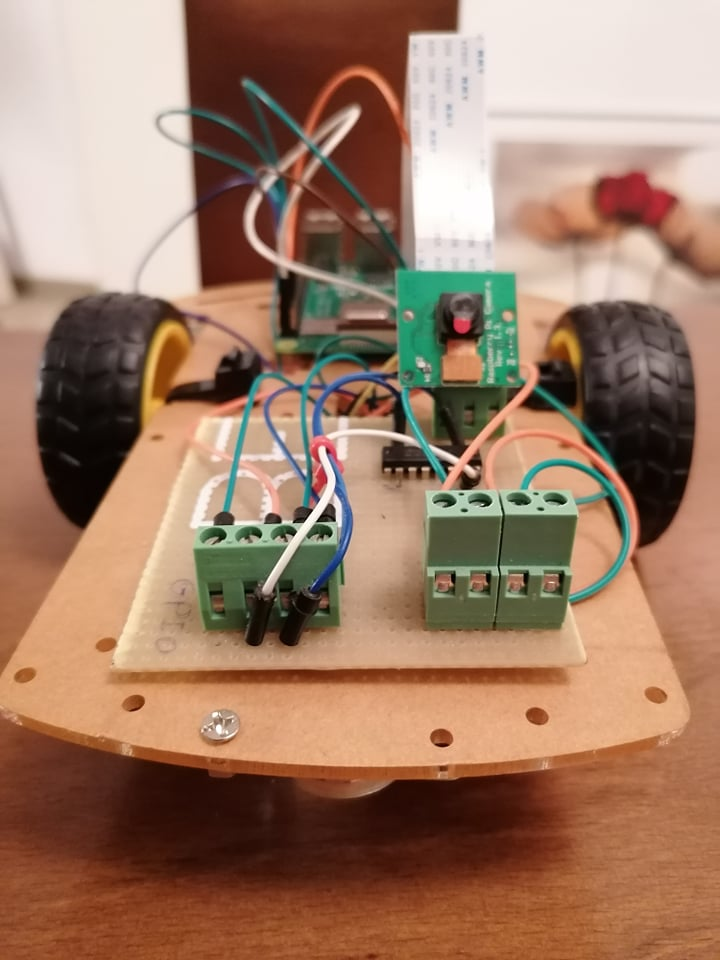
\includegraphics{robot.jpg}    

    
    IOT Raspberry PI und Python

Younes Labidi \& Moez Rjiba

    

    \hypertarget{inhalt}{%
\subsection{Inhalt :}\label{inhalt}}

\begin{itemize}
\tightlist
\item
  Framework installation
\item
  Python motors code
\item
  Kamera-Stream-Code mit Bewegungserkennung
\item
  HTML code
\end{itemize}

    \hypertarget{framework-installation}{%
\subsection{Framework installation :}\label{framework-installation}}

    \begin{tcolorbox}[breakable, size=fbox, boxrule=1pt, pad at break*=1mm,colback=cellbackground, colframe=cellborder]
\prompt{In}{incolor}{15}{\boxspacing}
\begin{Verbatim}[commandchars=\\\{\}]
\PY{o}{!} pip install Flask
\end{Verbatim}
\end{tcolorbox}

    \begin{Verbatim}[commandchars=\\\{\}]
Collecting Flask
  Using cached https://files.pythonhosted.org/packages/f2/28/2a03252dfb9ebf377f4
0fba6a7841b47083260bf8bd8e737b0c6952df83f/Flask-1.1.2-py2.py3-none-any.whl
Collecting click>=5.1 (from Flask)
  Using cached https://files.pythonhosted.org/packages/d2/3d/fa76db83bf75c4f8d33
8c2fd15c8d33fdd7ad23a9b5e57eb6c5de26b430e/click-7.1.2-py2.py3-none-any.whl
Collecting Werkzeug>=0.15 (from Flask)
  Using cached https://files.pythonhosted.org/packages/cc/94/5f7079a0e00bd6863ef
8f1da638721e9da21e5bacee597595b318f71d62e/Werkzeug-1.0.1-py2.py3-none-any.whl
Collecting itsdangerous>=0.24 (from Flask)
  Using cached https://files.pythonhosted.org/packages/76/ae/44b03b253d6fade317f
32c24d100b3b35c2239807046a4c953c7b89fa49e/itsdangerous-1.1.0-py2.py3-none-
any.whl
Collecting Jinja2>=2.10.1 (from Flask)
  Using cached https://files.pythonhosted.org/packages/30/9e/f663a2aa66a09d83804
2ae1a2c5659828bb9b41ea3a6efa20a20fd92b121/Jinja2-2.11.2-py2.py3-none-any.whl
Collecting MarkupSafe>=0.23 (from Jinja2>=2.10.1->Flask)
  Using cached https://files.pythonhosted.org/packages/fb/40/f3adb7cf24a8012813c
5edb20329eb22d5d8e2a0ecf73d21d6b85865da11/MarkupSafe-1.1.1-cp27-cp27mu-
manylinux1\_x86\_64.whl
Installing collected packages: click, Werkzeug, itsdangerous, MarkupSafe,
Jinja2, Flask
Successfully installed Flask-1.1.2 Jinja2-2.11.2 MarkupSafe-1.1.1 Werkzeug-1.0.1
click-7.1.2 itsdangerous-1.1.0
    \end{Verbatim}

    Flask ist ein Mikro-Web-Framework für unsere Web-Interface, mit dem wir
das Auto steuern und den Live-Stream abrufen können.

    \begin{tcolorbox}[breakable, size=fbox, boxrule=1pt, pad at break*=1mm,colback=cellbackground, colframe=cellborder]
\prompt{In}{incolor}{2}{\boxspacing}
\begin{Verbatim}[commandchars=\\\{\}]
\PY{o}{!} pip install numpy
\end{Verbatim}
\end{tcolorbox}

    \begin{Verbatim}[commandchars=\\\{\}]
Defaulting to user installation because normal site-packages is not writeable
Looking in indexes: https://pypi.org/simple, https://www.piwheels.org/simple
Requirement already satisfied: numpy in /usr/lib/python3/dist-packages (1.16.2)
    \end{Verbatim}

    Hier verwenden wir die numpy-Bibliothek zusätzlich mit opencv- und
imutils-Bibliotheken, um die Kamera auf die Web-Interface zu streamen.

    \begin{tcolorbox}[breakable, size=fbox, boxrule=1pt, pad at break*=1mm,colback=cellbackground, colframe=cellborder]
\prompt{In}{incolor}{4}{\boxspacing}
\begin{Verbatim}[commandchars=\\\{\}]
\PY{o}{!} pip install opencv\PYZhy{}python
\end{Verbatim}
\end{tcolorbox}

    \begin{Verbatim}[commandchars=\\\{\}]
Defaulting to user installation because normal site-packages is not writeable
Looking in indexes: https://pypi.org/simple, https://www.piwheels.org/simple
Requirement already satisfied: opencv-python in
/home/pi/.local/lib/python3.7/site-packages (4.1.1.26)
Requirement already satisfied: numpy>=1.16.2 in /usr/lib/python3/dist-packages
(from opencv-python) (1.16.2)
    \end{Verbatim}

    \begin{tcolorbox}[breakable, size=fbox, boxrule=1pt, pad at break*=1mm,colback=cellbackground, colframe=cellborder]
\prompt{In}{incolor}{5}{\boxspacing}
\begin{Verbatim}[commandchars=\\\{\}]
\PY{o}{!} pip install imutils
\end{Verbatim}
\end{tcolorbox}

    \begin{Verbatim}[commandchars=\\\{\}]
Defaulting to user installation because normal site-packages is not writeable
Looking in indexes: https://pypi.org/simple, https://www.piwheels.org/simple
Requirement already satisfied: imutils in /home/pi/.local/lib/python3.7/site-
packages (0.5.3)
    \end{Verbatim}

    \hypertarget{python-motors-code}{%
\section{Python motors code :}\label{python-motors-code}}

    Aufstellen von Pins an der Raspberry Pi zur Steuerung der Motoren.

    \begin{tcolorbox}[breakable, size=fbox, boxrule=1pt, pad at break*=1mm,colback=cellbackground, colframe=cellborder]
\prompt{In}{incolor}{1}{\boxspacing}
\begin{Verbatim}[commandchars=\\\{\}]
\PY{k+kn}{from} \PY{n+nn}{flask} \PY{k+kn}{import} \PY{n}{Flask}\PY{p}{,} \PY{n}{render\PYZus{}template}\PY{p}{,} \PY{n}{request}\PY{p}{,} \PY{n}{redirect}\PY{p}{,} \PY{n}{url\PYZus{}for}\PY{p}{,} \PY{n}{make\PYZus{}response} 
\PY{k+kn}{import} \PY{n+nn}{time}
\PY{k+kn}{import} \PY{n+nn}{RPi}\PY{n+nn}{.}\PY{n+nn}{GPIO} \PY{k}{as} \PY{n+nn}{GPIO}

\PY{n}{mA1}\PY{o}{=}\PY{l+m+mi}{18} \PY{c+c1}{\PYZsh{}Motor1}
\PY{n}{mA2}\PY{o}{=}\PY{l+m+mi}{23}
\PY{n}{mB1}\PY{o}{=}\PY{l+m+mi}{24} \PY{c+c1}{\PYZsh{}Motor2}
\PY{n}{mB2}\PY{o}{=}\PY{l+m+mi}{25}

\PY{n}{GPIO}\PY{o}{.}\PY{n}{setmode}\PY{p}{(}\PY{n}{GPIO}\PY{o}{.}\PY{n}{BCM}\PY{p}{)}    \PY{c+c1}{\PYZsh{}Referring to the pins by the \PYZdq{}Broadcom SOC channel\PYZdq{} number}

\PY{n}{GPIO}\PY{o}{.}\PY{n}{setup}\PY{p}{(}\PY{n}{mA1}\PY{p}{,} \PY{n}{GPIO}\PY{o}{.}\PY{n}{OUT}\PY{p}{)} \PY{c+c1}{\PYZsh{}Motors GPIO as OUTPUT}
\PY{n}{GPIO}\PY{o}{.}\PY{n}{setup}\PY{p}{(}\PY{n}{mA2}\PY{p}{,} \PY{n}{GPIO}\PY{o}{.}\PY{n}{OUT}\PY{p}{)}
\PY{n}{GPIO}\PY{o}{.}\PY{n}{setup}\PY{p}{(}\PY{n}{mB1}\PY{p}{,} \PY{n}{GPIO}\PY{o}{.}\PY{n}{OUT}\PY{p}{)}
\PY{n}{GPIO}\PY{o}{.}\PY{n}{setup}\PY{p}{(}\PY{n}{mB2}\PY{p}{,} \PY{n}{GPIO}\PY{o}{.}\PY{n}{OUT}\PY{p}{)}

\PY{n}{GPIO}\PY{o}{.}\PY{n}{output}\PY{p}{(}\PY{n}{mA1} \PY{p}{,} \PY{l+m+mi}{0}\PY{p}{)}      \PY{c+c1}{\PYZsh{}Initial values 0 }
\PY{n}{GPIO}\PY{o}{.}\PY{n}{output}\PY{p}{(}\PY{n}{mA2} \PY{p}{,} \PY{l+m+mi}{0}\PY{p}{)}
\PY{n}{GPIO}\PY{o}{.}\PY{n}{output}\PY{p}{(}\PY{n}{mB1}\PY{p}{,} \PY{l+m+mi}{0}\PY{p}{)}
\PY{n}{GPIO}\PY{o}{.}\PY{n}{output}\PY{p}{(}\PY{n}{mB2}\PY{p}{,} \PY{l+m+mi}{0}\PY{p}{)}

\PY{n}{app} \PY{o}{=} \PY{n}{Flask}\PY{p}{(}\PY{n+nv+vm}{\PYZus{}\PYZus{}name\PYZus{}\PYZus{}}\PY{p}{)}     \PY{c+c1}{\PYZsh{}set up flask server}
\end{Verbatim}
\end{tcolorbox}

    \begin{Verbatim}[commandchars=\\\{\}]

      
      
      
      
        ---------------------------------------------------------------------------

        ModuleNotFoundError                       Traceback (most recent call last)

        <ipython-input-1-ddaf1e51f673> in <module>
          1 from flask import Flask, render\_template, request, redirect, url\_for, make\_response
          2 import time
    ----> 3 import RPi.GPIO as GPIO
          4 
          5 mA1=18 \#Motor1


        ModuleNotFoundError: No module named 'RPi'

    \end{Verbatim}

    Normaler Fehler, da er auf einer Raspberry-PI und nicht auf einem
Desktop ausgeführt wird.

    \begin{tcolorbox}[breakable, size=fbox, boxrule=1pt, pad at break*=1mm,colback=cellbackground, colframe=cellborder]
\prompt{In}{incolor}{ }{\boxspacing}
\begin{Verbatim}[commandchars=\\\{\}]
\PY{n+nd}{@app}\PY{o}{.}\PY{n}{route}\PY{p}{(}\PY{l+s+s1}{\PYZsq{}}\PY{l+s+s1}{/}\PY{l+s+s1}{\PYZsq{}}\PY{p}{)}
\PY{k}{def} \PY{n+nf}{index}\PY{p}{(}\PY{p}{)}\PY{p}{:}
    \PY{k}{return} \PY{n}{render\PYZus{}template}\PY{p}{(}\PY{l+s+s1}{\PYZsq{}}\PY{l+s+s1}{index.html}\PY{l+s+s1}{\PYZsq{}}\PY{p}{)}

\PY{c+c1}{\PYZsh{}Recieve which pin to change from the button press on index.html}
\PY{c+c1}{\PYZsh{}Each button returns a number that triggers a command in this function}
\end{Verbatim}
\end{tcolorbox}

    \begin{tcolorbox}[breakable, size=fbox, boxrule=1pt, pad at break*=1mm,colback=cellbackground, colframe=cellborder]
\prompt{In}{incolor}{ }{\boxspacing}
\begin{Verbatim}[commandchars=\\\{\}]
\PY{c+c1}{\PYZsh{}Uses methods from motors.py to send commands to the GPIO to operate the motors}
\PY{n+nd}{@app}\PY{o}{.}\PY{n}{route}\PY{p}{(}\PY{l+s+s1}{\PYZsq{}}\PY{l+s+s1}{/\PYZlt{}changepin\PYZgt{}}\PY{l+s+s1}{\PYZsq{}}\PY{p}{,} \PY{n}{methods}\PY{o}{=}\PY{p}{[}\PY{l+s+s1}{\PYZsq{}}\PY{l+s+s1}{POST}\PY{l+s+s1}{\PYZsq{}}\PY{p}{]}\PY{p}{)}
\PY{k}{def} \PY{n+nf}{reroute}\PY{p}{(}\PY{n}{changepin}\PY{p}{)}\PY{p}{:}
    \PY{n}{changePin} \PY{o}{=} \PY{n+nb}{int}\PY{p}{(}\PY{n}{changepin}\PY{p}{)} \PY{c+c1}{\PYZsh{}cast changepin to an int}
    \PY{k}{if} \PY{n}{changePin} \PY{o}{==} \PY{l+m+mi}{1}\PY{p}{:}
        \PY{n+nb}{print} \PY{p}{(}\PY{l+s+s2}{\PYZdq{}}\PY{l+s+s2}{Vorne}\PY{l+s+s2}{\PYZdq{}}\PY{p}{)} \PY{c+c1}{\PYZsh{} drive forward}
        \PY{n}{GPIO}\PY{o}{.}\PY{n}{output}\PY{p}{(}\PY{n}{mA1} \PY{p}{,} \PY{l+m+mi}{0}\PY{p}{)}
        \PY{n}{GPIO}\PY{o}{.}\PY{n}{output}\PY{p}{(}\PY{n}{mA2} \PY{p}{,} \PY{l+m+mi}{1}\PY{p}{)}
        \PY{n}{GPIO}\PY{o}{.}\PY{n}{output}\PY{p}{(}\PY{n}{mB1} \PY{p}{,} \PY{l+m+mi}{1}\PY{p}{)}
        \PY{n}{GPIO}\PY{o}{.}\PY{n}{output}\PY{p}{(}\PY{n}{mB2} \PY{p}{,} \PY{l+m+mi}{0}\PY{p}{)}
    \PY{k}{elif} \PY{n}{changePin} \PY{o}{==} \PY{l+m+mi}{2}\PY{p}{:}
        \PY{n+nb}{print} \PY{p}{(}\PY{l+s+s2}{\PYZdq{}}\PY{l+s+s2}{Links}\PY{l+s+s2}{\PYZdq{}}\PY{p}{)} \PY{c+c1}{\PYZsh{} turn left}
        \PY{n}{GPIO}\PY{o}{.}\PY{n}{output}\PY{p}{(}\PY{n}{mA1} \PY{p}{,} \PY{l+m+mi}{0}\PY{p}{)}
        \PY{n}{GPIO}\PY{o}{.}\PY{n}{output}\PY{p}{(}\PY{n}{mA2} \PY{p}{,} \PY{l+m+mi}{0}\PY{p}{)}
        \PY{n}{GPIO}\PY{o}{.}\PY{n}{output}\PY{p}{(}\PY{n}{mB1} \PY{p}{,} \PY{l+m+mi}{1}\PY{p}{)}
        \PY{n}{GPIO}\PY{o}{.}\PY{n}{output}\PY{p}{(}\PY{n}{mB2} \PY{p}{,} \PY{l+m+mi}{0}\PY{p}{)}
    \PY{k}{elif} \PY{n}{changePin} \PY{o}{==} \PY{l+m+mi}{3}\PY{p}{:}
        \PY{n+nb}{print} \PY{p}{(}\PY{l+s+s2}{\PYZdq{}}\PY{l+s+s2}{Stop}\PY{l+s+s2}{\PYZdq{}}\PY{p}{)} \PY{c+c1}{\PYZsh{} stop the car}
        \PY{n}{GPIO}\PY{o}{.}\PY{n}{output}\PY{p}{(}\PY{n}{mA1} \PY{p}{,} \PY{l+m+mi}{0}\PY{p}{)}
        \PY{n}{GPIO}\PY{o}{.}\PY{n}{output}\PY{p}{(}\PY{n}{mA2} \PY{p}{,} \PY{l+m+mi}{0}\PY{p}{)}
        \PY{n}{GPIO}\PY{o}{.}\PY{n}{output}\PY{p}{(}\PY{n}{mB1} \PY{p}{,} \PY{l+m+mi}{0}\PY{p}{)}
        \PY{n}{GPIO}\PY{o}{.}\PY{n}{output}\PY{p}{(}\PY{n}{mB2} \PY{p}{,} \PY{l+m+mi}{0}\PY{p}{)}
    \PY{k}{elif} \PY{n}{changePin} \PY{o}{==} \PY{l+m+mi}{4}\PY{p}{:}
        \PY{n+nb}{print} \PY{p}{(}\PY{l+s+s2}{\PYZdq{}}\PY{l+s+s2}{Rechts}\PY{l+s+s2}{\PYZdq{}}\PY{p}{)} \PY{c+c1}{\PYZsh{} turn right}
        \PY{n}{GPIO}\PY{o}{.}\PY{n}{output}\PY{p}{(}\PY{n}{mA1} \PY{p}{,} \PY{l+m+mi}{0}\PY{p}{)}
        \PY{n}{GPIO}\PY{o}{.}\PY{n}{output}\PY{p}{(}\PY{n}{mA2} \PY{p}{,} \PY{l+m+mi}{1}\PY{p}{)}
        \PY{n}{GPIO}\PY{o}{.}\PY{n}{output}\PY{p}{(}\PY{n}{mB1} \PY{p}{,} \PY{l+m+mi}{0}\PY{p}{)}
        \PY{n}{GPIO}\PY{o}{.}\PY{n}{output}\PY{p}{(}\PY{n}{mB2} \PY{p}{,} \PY{l+m+mi}{0}\PY{p}{)}
    \PY{k}{else}\PY{p}{:}
        \PY{n+nb}{print}\PY{p}{(}\PY{l+s+s2}{\PYZdq{}}\PY{l+s+s2}{Reverse}\PY{l+s+s2}{\PYZdq{}}\PY{p}{)} \PY{c+c1}{\PYZsh{} drive backwards}
        \PY{n}{GPIO}\PY{o}{.}\PY{n}{output}\PY{p}{(}\PY{n}{mA1} \PY{p}{,} \PY{l+m+mi}{1}\PY{p}{)}
        \PY{n}{GPIO}\PY{o}{.}\PY{n}{output}\PY{p}{(}\PY{n}{mA2} \PY{p}{,} \PY{l+m+mi}{0}\PY{p}{)}
        \PY{n}{GPIO}\PY{o}{.}\PY{n}{output}\PY{p}{(}\PY{n}{mB1} \PY{p}{,} \PY{l+m+mi}{0}\PY{p}{)}
        \PY{n}{GPIO}\PY{o}{.}\PY{n}{output}\PY{p}{(}\PY{n}{mB2} \PY{p}{,} \PY{l+m+mi}{1}\PY{p}{)}
    \PY{n}{response} \PY{o}{=} \PY{n}{make\PYZus{}response}\PY{p}{(}\PY{n}{redirect}\PY{p}{(}\PY{n}{url\PYZus{}for}\PY{p}{(}\PY{l+s+s1}{\PYZsq{}}\PY{l+s+s1}{index}\PY{l+s+s1}{\PYZsq{}}\PY{p}{)}\PY{p}{)}\PY{p}{)}
    \PY{k}{return}\PY{p}{(}\PY{n}{response}\PY{p}{)}
\PY{n}{app}\PY{o}{.}\PY{n}{run}\PY{p}{(}\PY{n}{debug}\PY{o}{=}\PY{k+kc}{True}\PY{p}{,} \PY{n}{host}\PY{o}{=}\PY{l+s+s1}{\PYZsq{}}\PY{l+s+s1}{0.0.0.0}\PY{l+s+s1}{\PYZsq{}}\PY{p}{,} \PY{n}{port}\PY{o}{=}\PY{l+m+mi}{8000}\PY{p}{)} \PY{c+c1}{\PYZsh{}set up the server in debug mode to the port 8000}
\end{Verbatim}
\end{tcolorbox}

    \hypertarget{kamera-stream-code-mit-bewegungserkennung}{%
\section{Kamera-Stream-Code mit Bewegungserkennung
:}\label{kamera-stream-code-mit-bewegungserkennung}}

        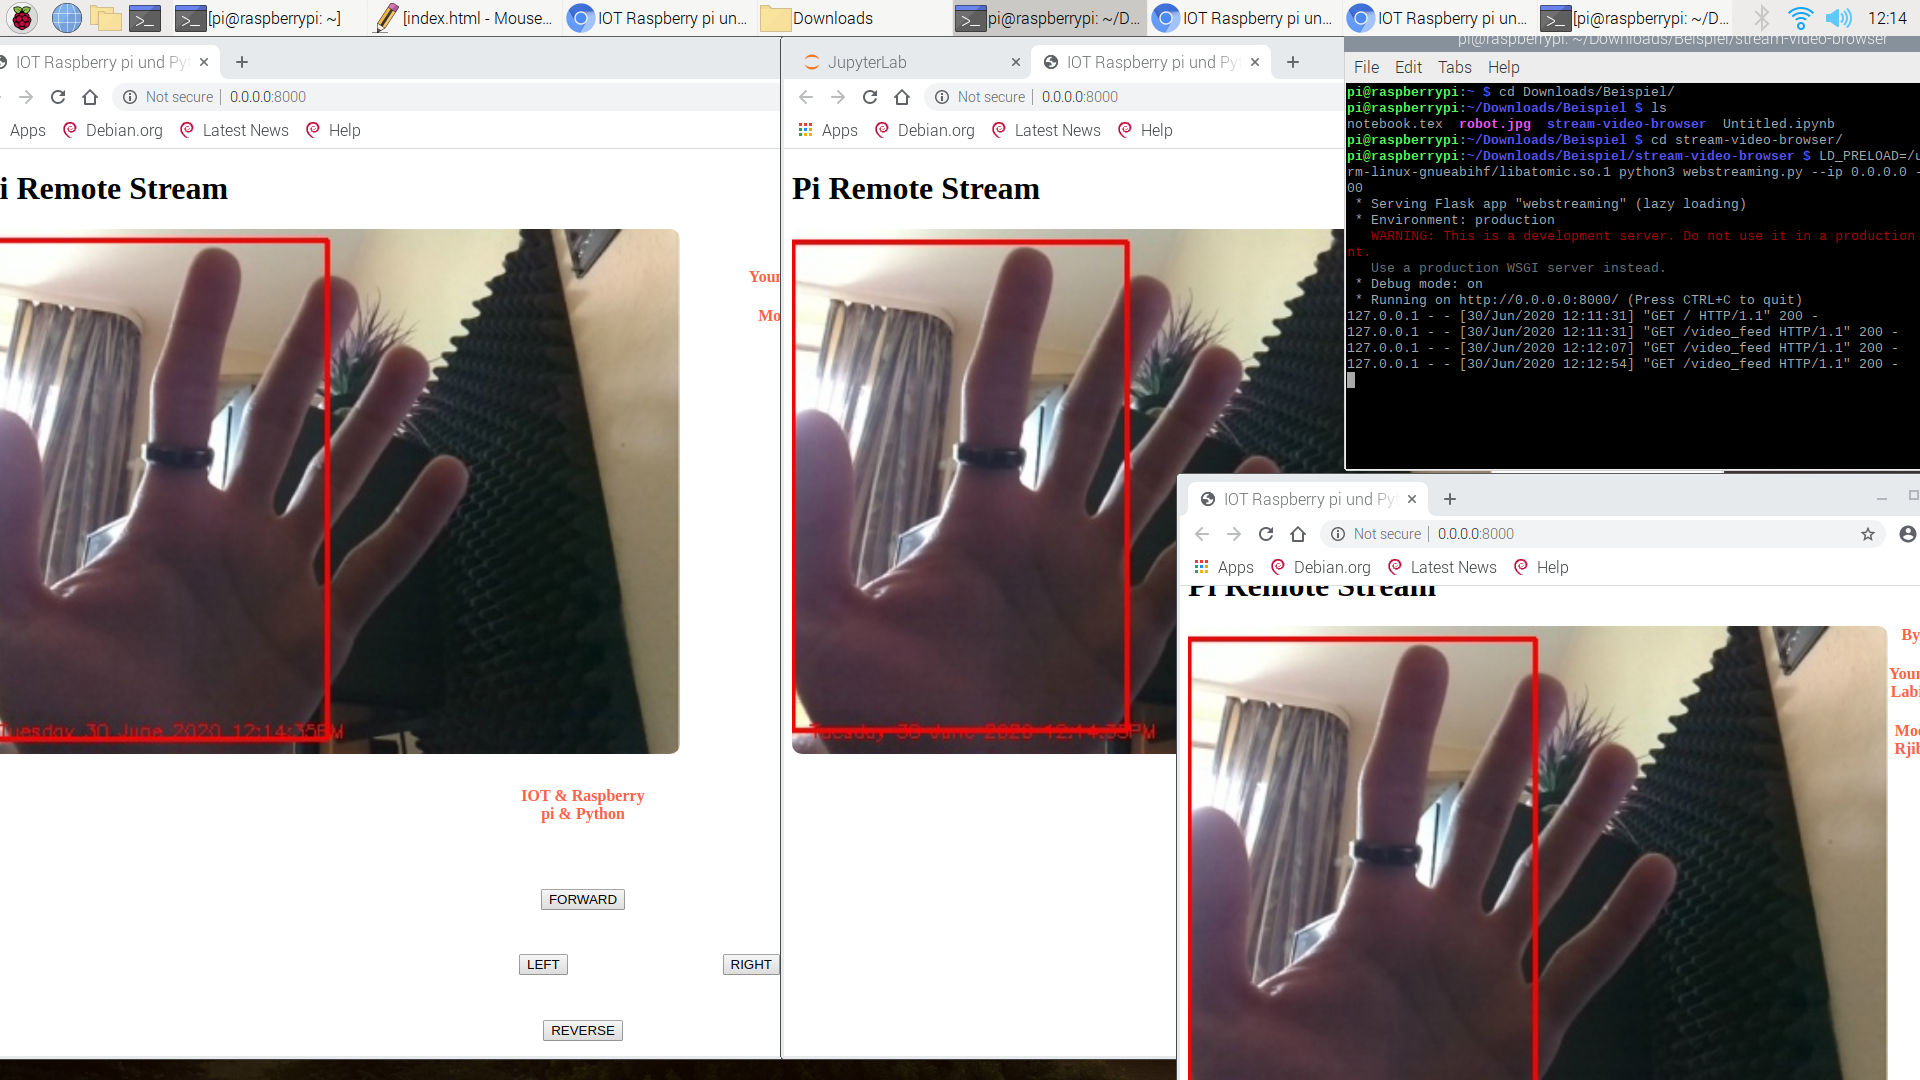
\includegraphics[width=18cm]{2020-06-30-121435_1920x1080_scrot.png}


    Bewegungserkennungsalgorithmus, der Numpy für die numerische
Verarbeitung, Imutils für unsere Komfortfunktionen und cv2 für
OpenCV-Bindungen verwendet.

    Unser Bewegungsmelder-Algorithmus erkennt Bewegung durch eine Form der
Hintergrundsubtraktion.

Der Subtraktionsalgorithmus arbeitet nach:

\begin{verbatim}
1- Akkumulieren des gewichteten Mittelwertes der vorherigen N Bilder.
2- Nehmen Sie den aktuellen Rahmen und subtrahieren Sie ihn vom gewichteten Durchschnitt
der Rahmen.
3- Schwellenwert für die Ausgabe der Subtraktion, um die Regionen mit erheblichen 
Unterschieden in den Pixelwerten hervorzuheben 
("weiß" für den Vordergrund und "schwarz" für den Hintergrund).
4- Anwendung grundlegender Bildverarbeitungstechniken wie Erosionen und Dilatationen, 
um Rauschen zu entfernen.
5- Verwendung der Konturerkennung zur Extraktion der Regionen, die eine Bewegung enthalten.
\end{verbatim}

    Unsere Bewegungserkennungs-Implementierung wird innerhalb der
SingleMotionDetector-Klasse leben, die in singleMotionDetector.py zu
finden ist.

Sie wird als ``Einzelbewegungsmelder'' bezeichnet, da der Algorithmus
selbst nur daran interessiert ist, die größte einzelne Bewegungsregion
zu finden.

Wir können diese Methode leicht erweitern, um auch mehrere
Bewegungsregionen zu behandeln.

    \begin{tcolorbox}[breakable, size=fbox, boxrule=1pt, pad at break*=1mm,colback=cellbackground, colframe=cellborder]
\prompt{In}{incolor}{8}{\boxspacing}
\begin{Verbatim}[commandchars=\\\{\}]
\PY{c+c1}{\PYZsh{} import the necessary packages}
\PY{k+kn}{import} \PY{n+nn}{numpy} \PY{k}{as} \PY{n+nn}{np}
\PY{k+kn}{import} \PY{n+nn}{imutils}
\PY{k+kn}{import} \PY{n+nn}{cv2}
\end{Verbatim}
\end{tcolorbox}

    \begin{Verbatim}[commandchars=\\\{\}]

      
      
      
      
        ---------------------------------------------------------------------------

        ImportError                               Traceback (most recent call last)

        <ipython-input-8-ea8c565de04b> in <module>
          1 \# import the necessary packages
          2 import numpy as np
    ----> 3 import imutils
          4 import cv2


        \textasciitilde{}/.local/lib/python3.7/site-packages/imutils/\_\_init\_\_.py in <module>
          6 
          7 \# import the necessary packages
    ----> 8 from .convenience import translate
          9 from .convenience import rotate
         10 from .convenience import rotate\_bound


        \textasciitilde{}/.local/lib/python3.7/site-packages/imutils/convenience.py in <module>
          4 \# import the necessary packages
          5 import numpy as np
    ----> 6 import cv2
          7 import sys
          8 


        \textasciitilde{}/.local/lib/python3.7/site-packages/cv2/\_\_init\_\_.py in <module>
          1 import importlib
          2 
    ----> 3 from .cv2 import *
          4 from .data import *
          5 


        ImportError: /home/pi/.local/lib/python3.7/site-packages/cv2/cv2.cpython-37m-arm-linux-gnueabihf.so: undefined symbol: \_\_atomic\_fetch\_add\_8

    \end{Verbatim}

    Wenn Sie diesen Importfehler erhalten, führen Sie Ihr Programm einfach
mit diesem Befehl aus:

LD\_PRELOAD=/usr/lib/arm-linux-gnueabihf/libatomic.so.1 python3
webstreaming.py --ip 0.0.0.0 --port 8000

    \begin{tcolorbox}[breakable, size=fbox, boxrule=1pt, pad at break*=1mm,colback=cellbackground, colframe=cellborder]
\prompt{In}{incolor}{9}{\boxspacing}
\begin{Verbatim}[commandchars=\\\{\}]
\PY{k}{class} \PY{n+nc}{SingleMotionDetector}\PY{p}{:}
    \PY{k}{def} \PY{n+nf+fm}{\PYZus{}\PYZus{}init\PYZus{}\PYZus{}}\PY{p}{(}\PY{n+nb+bp}{self}\PY{p}{,} \PY{n}{accumWeight}\PY{o}{=}\PY{l+m+mf}{0.5}\PY{p}{)}\PY{p}{:}
        \PY{c+c1}{\PYZsh{} store the accumulated weight factor}
        \PY{n+nb+bp}{self}\PY{o}{.}\PY{n}{accumWeight} \PY{o}{=} \PY{n}{accumWeight}

        \PY{c+c1}{\PYZsh{} initialize the background model}
        \PY{n+nb+bp}{self}\PY{o}{.}\PY{n}{bg} \PY{o}{=} \PY{k+kc}{None}
\end{Verbatim}
\end{tcolorbox}

    Je größer accumWeight ist, desto weniger wird der Hintergrund (bg) bei
der Akkumulation des gewichteten Durchschnitts berücksichtigt.

    \begin{tcolorbox}[breakable, size=fbox, boxrule=1pt, pad at break*=1mm,colback=cellbackground, colframe=cellborder]
\prompt{In}{incolor}{ }{\boxspacing}
\begin{Verbatim}[commandchars=\\\{\}]
    \PY{k}{def} \PY{n+nf}{update}\PY{p}{(}\PY{n+nb+bp}{self}\PY{p}{,} \PY{n}{image}\PY{p}{)}\PY{p}{:}
        \PY{c+c1}{\PYZsh{} if the background model is None, initialize it}
        \PY{k}{if} \PY{n+nb+bp}{self}\PY{o}{.}\PY{n}{bg} \PY{o+ow}{is} \PY{k+kc}{None}\PY{p}{:}
            \PY{n+nb+bp}{self}\PY{o}{.}\PY{n}{bg} \PY{o}{=} \PY{n}{image}\PY{o}{.}\PY{n}{copy}\PY{p}{(}\PY{p}{)}\PY{o}{.}\PY{n}{astype}\PY{p}{(}\PY{l+s+s2}{\PYZdq{}}\PY{l+s+s2}{float}\PY{l+s+s2}{\PYZdq{}}\PY{p}{)}
            \PY{k}{return}

        \PY{c+c1}{\PYZsh{} update the background model by accumulating the weighted}
        \PY{c+c1}{\PYZsh{} average}
        \PY{n}{cv2}\PY{o}{.}\PY{n}{accumulateWeighted}\PY{p}{(}\PY{n}{image}\PY{p}{,} \PY{n+nb+bp}{self}\PY{o}{.}\PY{n}{bg}\PY{p}{,} \PY{n+nb+bp}{self}\PY{o}{.}\PY{n}{accumWeight}\PY{p}{)}
\end{Verbatim}
\end{tcolorbox}

    Definiert eine Aktualisierungsmethode, die ein Eingabefenster akzeptiert
und den gewichteten Durchschnitt berechnet.

    \begin{tcolorbox}[breakable, size=fbox, boxrule=1pt, pad at break*=1mm,colback=cellbackground, colframe=cellborder]
\prompt{In}{incolor}{ }{\boxspacing}
\begin{Verbatim}[commandchars=\\\{\}]
    \PY{k}{def} \PY{n+nf}{detect}\PY{p}{(}\PY{n+nb+bp}{self}\PY{p}{,} \PY{n}{image}\PY{p}{,} \PY{n}{tVal}\PY{o}{=}\PY{l+m+mi}{25}\PY{p}{)}\PY{p}{:}
        \PY{c+c1}{\PYZsh{} compute the absolute difference between the background model}
        \PY{c+c1}{\PYZsh{} and the image passed in, then threshold the delta image}
        \PY{n}{delta} \PY{o}{=} \PY{n}{cv2}\PY{o}{.}\PY{n}{absdiff}\PY{p}{(}\PY{n+nb+bp}{self}\PY{o}{.}\PY{n}{bg}\PY{o}{.}\PY{n}{astype}\PY{p}{(}\PY{l+s+s2}{\PYZdq{}}\PY{l+s+s2}{uint8}\PY{l+s+s2}{\PYZdq{}}\PY{p}{)}\PY{p}{,} \PY{n}{image}\PY{p}{)}
        \PY{n}{thresh} \PY{o}{=} \PY{n}{cv2}\PY{o}{.}\PY{n}{threshold}\PY{p}{(}\PY{n}{delta}\PY{p}{,} \PY{n}{tVal}\PY{p}{,} \PY{l+m+mi}{255}\PY{p}{,} \PY{n}{cv2}\PY{o}{.}\PY{n}{THRESH\PYZus{}BINARY}\PY{p}{)}\PY{p}{[}\PY{l+m+mi}{1}\PY{p}{]}

        \PY{c+c1}{\PYZsh{} perform a series of erosions and dilations to remove small}
        \PY{c+c1}{\PYZsh{} blobs}
        \PY{n}{thresh} \PY{o}{=} \PY{n}{cv2}\PY{o}{.}\PY{n}{erode}\PY{p}{(}\PY{n}{thresh}\PY{p}{,} \PY{k+kc}{None}\PY{p}{,} \PY{n}{iterations}\PY{o}{=}\PY{l+m+mi}{2}\PY{p}{)}
        \PY{n}{thresh} \PY{o}{=} \PY{n}{cv2}\PY{o}{.}\PY{n}{dilate}\PY{p}{(}\PY{n}{thresh}\PY{p}{,} \PY{k+kc}{None}\PY{p}{,} \PY{n}{iterations}\PY{o}{=}\PY{l+m+mi}{2}\PY{p}{)}
        

  
        
\end{Verbatim}
\end{tcolorbox}

    Vor unserem Hintergrund (bg) können wir nun die Bewegungserkennung
mittels Detektionsmethode anwenden.

Die Methode erfordert einen einzigen Parameter mit einem optionalen
Parameter:

\begin{verbatim}
    -image: Eingabebild
    -tval : Schwellenwert
\end{verbatim}

    \begin{tcolorbox}[breakable, size=fbox, boxrule=1pt, pad at break*=1mm,colback=cellbackground, colframe=cellborder]
\prompt{In}{incolor}{ }{\boxspacing}
\begin{Verbatim}[commandchars=\\\{\}]
        \PY{c+c1}{\PYZsh{} find contours in the thresholded image and initialize the}
        \PY{c+c1}{\PYZsh{} minimum and maximum bounding box regions for motion}
        \PY{n}{cnts} \PY{o}{=} \PY{n}{cv2}\PY{o}{.}\PY{n}{findContours}\PY{p}{(}\PY{n}{thresh}\PY{o}{.}\PY{n}{copy}\PY{p}{(}\PY{p}{)}\PY{p}{,} \PY{n}{cv2}\PY{o}{.}\PY{n}{RETR\PYZus{}EXTERNAL}\PY{p}{,}
            \PY{n}{cv2}\PY{o}{.}\PY{n}{CHAIN\PYZus{}APPROX\PYZus{}SIMPLE}\PY{p}{)}
        \PY{n}{cnts} \PY{o}{=} \PY{n}{imutils}\PY{o}{.}\PY{n}{grab\PYZus{}contours}\PY{p}{(}\PY{n}{cnts}\PY{p}{)}
        \PY{p}{(}\PY{n}{minX}\PY{p}{,} \PY{n}{minY}\PY{p}{)} \PY{o}{=} \PY{p}{(}\PY{n}{np}\PY{o}{.}\PY{n}{inf}\PY{p}{,} \PY{n}{np}\PY{o}{.}\PY{n}{inf}\PY{p}{)}
        \PY{p}{(}\PY{n}{maxX}\PY{p}{,} \PY{n}{maxY}\PY{p}{)} \PY{o}{=} \PY{p}{(}\PY{o}{\PYZhy{}}\PY{n}{np}\PY{o}{.}\PY{n}{inf}\PY{p}{,} \PY{o}{\PYZhy{}}\PY{n}{np}\PY{o}{.}\PY{n}{inf}\PY{p}{)}
\end{Verbatim}
\end{tcolorbox}

    Anwendung der Konturerkennung zum Extrahieren beliebiger Bewegungen.

    \begin{tcolorbox}[breakable, size=fbox, boxrule=1pt, pad at break*=1mm,colback=cellbackground, colframe=cellborder]
\prompt{In}{incolor}{ }{\boxspacing}
\begin{Verbatim}[commandchars=\\\{\}]
 \PY{c+c1}{\PYZsh{} if no contours were found, return None}
        \PY{k}{if} \PY{n+nb}{len}\PY{p}{(}\PY{n}{cnts}\PY{p}{)} \PY{o}{==} \PY{l+m+mi}{0}\PY{p}{:}
            \PY{k}{return} \PY{k+kc}{None}

        \PY{c+c1}{\PYZsh{} otherwise, loop over the contours}
        \PY{k}{for} \PY{n}{c} \PY{o+ow}{in} \PY{n}{cnts}\PY{p}{:}
            \PY{c+c1}{\PYZsh{} compute the bounding box of the contour and use it to}
            \PY{c+c1}{\PYZsh{} update the minimum and maximum bounding box regions}
            \PY{p}{(}\PY{n}{x}\PY{p}{,} \PY{n}{y}\PY{p}{,} \PY{n}{w}\PY{p}{,} \PY{n}{h}\PY{p}{)} \PY{o}{=} \PY{n}{cv2}\PY{o}{.}\PY{n}{boundingRect}\PY{p}{(}\PY{n}{c}\PY{p}{)}
            \PY{p}{(}\PY{n}{minX}\PY{p}{,} \PY{n}{minY}\PY{p}{)} \PY{o}{=} \PY{p}{(}\PY{n+nb}{min}\PY{p}{(}\PY{n}{minX}\PY{p}{,} \PY{n}{x}\PY{p}{)}\PY{p}{,} \PY{n+nb}{min}\PY{p}{(}\PY{n}{minY}\PY{p}{,} \PY{n}{y}\PY{p}{)}\PY{p}{)}
            \PY{p}{(}\PY{n}{maxX}\PY{p}{,} \PY{n}{maxY}\PY{p}{)} \PY{o}{=} \PY{p}{(}\PY{n+nb}{max}\PY{p}{(}\PY{n}{maxX}\PY{p}{,} \PY{n}{x} \PY{o}{+} \PY{n}{w}\PY{p}{)}\PY{p}{,} \PY{n+nb}{max}\PY{p}{(}\PY{n}{maxY}\PY{p}{,} \PY{n}{y} \PY{o}{+} \PY{n}{h}\PY{p}{)}\PY{p}{)}

        \PY{c+c1}{\PYZsh{} otherwise, return a tuple of the thresholded image along}
        \PY{c+c1}{\PYZsh{} with bounding box}
        \PY{k}{return} \PY{p}{(}\PY{n}{thresh}\PY{p}{,} \PY{p}{(}\PY{n}{minX}\PY{p}{,} \PY{n}{minY}\PY{p}{,} \PY{n}{maxX}\PY{p}{,} \PY{n}{maxY}\PY{p}{)}\PY{p}{)}
\end{Verbatim}
\end{tcolorbox}

    Wir prüfen, ob unsere Konturenliste leer ist.

Wenn das der Fall ist, dann wurde keine Bewegung im Rahmen gefunden, und
wir können sie getrost ignorieren.

    \hypertarget{init}{%
\section{Init}\label{init}}

    \begin{tcolorbox}[breakable, size=fbox, boxrule=1pt, pad at break*=1mm,colback=cellbackground, colframe=cellborder]
\prompt{In}{incolor}{ }{\boxspacing}
\begin{Verbatim}[commandchars=\\\{\}]
\PY{c+c1}{\PYZsh{} import the necessary packages}
\PY{k+kn}{from} \PY{n+nn}{.}\PY{n+nn}{singlemotiondetector} \PY{k+kn}{import} \PY{n}{SingleMotionDetector}
\end{Verbatim}
\end{tcolorbox}

    \hypertarget{kombination-von-opencv-mit-flask}{%
\section{Kombination von OpenCV mit
Flask}\label{kombination-von-opencv-mit-flask}}

    Import unseres Bewegungserkennungsalgorithmus, Flask zum Rendern unserer
index.html-Vorlage und Threading, damit wir Gleichzeitigkeit
unterstützen können.

    \begin{tcolorbox}[breakable, size=fbox, boxrule=1pt, pad at break*=1mm,colback=cellbackground, colframe=cellborder]
\prompt{In}{incolor}{ }{\boxspacing}
\begin{Verbatim}[commandchars=\\\{\}]
\PY{c+c1}{\PYZsh{} USAGE}
\PY{c+c1}{\PYZsh{} python webstreaming.py \PYZhy{}\PYZhy{}ip 0.0.0.0 \PYZhy{}\PYZhy{}port 8000}

\PY{c+c1}{\PYZsh{} import the necessary packages}
\PY{k+kn}{from} \PY{n+nn}{pyimagesearch}\PY{n+nn}{.}\PY{n+nn}{motion\PYZus{}detection} \PY{k+kn}{import} \PY{n}{SingleMotionDetector}
\PY{k+kn}{from} \PY{n+nn}{imutils}\PY{n+nn}{.}\PY{n+nn}{video} \PY{k+kn}{import} \PY{n}{VideoStream}
\PY{k+kn}{from} \PY{n+nn}{flask} \PY{k+kn}{import} \PY{n}{Response}
\PY{k+kn}{from} \PY{n+nn}{flask} \PY{k+kn}{import} \PY{n}{Flask}
\PY{k+kn}{from} \PY{n+nn}{flask} \PY{k+kn}{import} \PY{n}{render\PYZus{}template}
\PY{k+kn}{import} \PY{n+nn}{threading}
\PY{k+kn}{import} \PY{n+nn}{argparse}
\PY{k+kn}{import} \PY{n+nn}{datetime}
\PY{k+kn}{import} \PY{n+nn}{imutils}
\PY{k+kn}{import} \PY{n+nn}{time}
\PY{k+kn}{import} \PY{n+nn}{cv2}
\end{Verbatim}
\end{tcolorbox}

    Kombination von OpenCV und Flask zur Bereitstellung von Einzelbildern
aus einem Videostream an einen Webbrowser.

    \begin{tcolorbox}[breakable, size=fbox, boxrule=1pt, pad at break*=1mm,colback=cellbackground, colframe=cellborder]
\prompt{In}{incolor}{ }{\boxspacing}
\begin{Verbatim}[commandchars=\\\{\}]
\PY{c+c1}{\PYZsh{} initialize the output frame and a lock used to ensure thread\PYZhy{}safe}
\PY{c+c1}{\PYZsh{} exchanges of the output frames (useful for multiple browsers/tabs}
\PY{c+c1}{\PYZsh{} are viewing tthe stream)}
\PY{n}{outputFrame} \PY{o}{=} \PY{k+kc}{None}
\PY{n}{lock} \PY{o}{=} \PY{n}{threading}\PY{o}{.}\PY{n}{Lock}\PY{p}{(}\PY{p}{)}

\PY{c+c1}{\PYZsh{} initialize a flask object}
\PY{n}{app} \PY{o}{=} \PY{n}{Flask}\PY{p}{(}\PY{n+nv+vm}{\PYZus{}\PYZus{}name\PYZus{}\PYZus{}}\PY{p}{)}

\PY{c+c1}{\PYZsh{} initialize the video stream and allow the camera sensor to}
\PY{c+c1}{\PYZsh{} warmup}
\PY{n}{vs} \PY{o}{=} \PY{n}{VideoStream}\PY{p}{(}\PY{n}{usePiCamera}\PY{o}{=}\PY{l+m+mi}{1}\PY{p}{)}\PY{o}{.}\PY{n}{start}\PY{p}{(}\PY{p}{)}
\PY{n}{time}\PY{o}{.}\PY{n}{sleep}\PY{p}{(}\PY{l+m+mf}{2.0}\PY{p}{)}
\end{Verbatim}
\end{tcolorbox}

    Initialisierung von outputFrame, derselbe Rahmen, der auch den Kunden
zur Verfügung gestellt wird.

Erstellen einer Sperre, um thread-sicheres Verhalten bei der
Aktualisierung des outputFrame zu gewährleisten.

Initialisierung der Flask-Anwendung beim Zugriff auf den Videostream.

    \begin{tcolorbox}[breakable, size=fbox, boxrule=1pt, pad at break*=1mm,colback=cellbackground, colframe=cellborder]
\prompt{In}{incolor}{ }{\boxspacing}
\begin{Verbatim}[commandchars=\\\{\}]
\PY{n+nd}{@app}\PY{o}{.}\PY{n}{route}\PY{p}{(}\PY{l+s+s2}{\PYZdq{}}\PY{l+s+s2}{/}\PY{l+s+s2}{\PYZdq{}}\PY{p}{)}
\PY{k}{def} \PY{n+nf}{index}\PY{p}{(}\PY{p}{)}\PY{p}{:}
    \PY{c+c1}{\PYZsh{} return the rendered template}
    \PY{k}{return} \PY{n}{render\PYZus{}template}\PY{p}{(}\PY{l+s+s2}{\PYZdq{}}\PY{l+s+s2}{index.html}\PY{l+s+s2}{\PYZdq{}}\PY{p}{)}
\end{Verbatim}
\end{tcolorbox}

    Rendern der index.html-Vorlage und Bereitstellen des
Ausgabe-Videostroms.

    \begin{tcolorbox}[breakable, size=fbox, boxrule=1pt, pad at break*=1mm,colback=cellbackground, colframe=cellborder]
\prompt{In}{incolor}{ }{\boxspacing}
\begin{Verbatim}[commandchars=\\\{\}]
\PY{k}{def} \PY{n+nf}{detect\PYZus{}motion}\PY{p}{(}\PY{n}{frameCount}\PY{p}{)}\PY{p}{:}
    \PY{c+c1}{\PYZsh{} grab global references to the video stream, output frame, and}
    \PY{c+c1}{\PYZsh{} lock variables}
    \PY{k}{global} \PY{n}{vs}\PY{p}{,} \PY{n}{outputFrame}\PY{p}{,} \PY{n}{lock}

    \PY{c+c1}{\PYZsh{} initialize the motion detector and the total number of frames}
    \PY{c+c1}{\PYZsh{} read thus far}
    \PY{n}{md} \PY{o}{=} \PY{n}{SingleMotionDetector}\PY{p}{(}\PY{n}{accumWeight}\PY{o}{=}\PY{l+m+mf}{0.1}\PY{p}{)}
    \PY{n}{total} \PY{o}{=} \PY{l+m+mi}{0}
\end{Verbatim}
\end{tcolorbox}

    Diese Funktion wird verantwortlich sein:

\begin{verbatim}
-Schleifen über Einzelbilder aus dem Videostrom
-Anwendung der Bewegungserkennung
-Zeichnungsergebnisse auf dem Ausgabeframe
\end{verbatim}

    \begin{tcolorbox}[breakable, size=fbox, boxrule=1pt, pad at break*=1mm,colback=cellbackground, colframe=cellborder]
\prompt{In}{incolor}{ }{\boxspacing}
\begin{Verbatim}[commandchars=\\\{\}]
    \PY{c+c1}{\PYZsh{} loop over frames from the video stream}
    \PY{k}{while} \PY{k+kc}{True}\PY{p}{:}
        \PY{c+c1}{\PYZsh{} read the next frame from the video stream, resize it,}
        \PY{c+c1}{\PYZsh{} convert the frame to grayscale, and blur it}
        \PY{n}{frame} \PY{o}{=} \PY{n}{vs}\PY{o}{.}\PY{n}{read}\PY{p}{(}\PY{p}{)}
        \PY{n}{frame} \PY{o}{=} \PY{n}{imutils}\PY{o}{.}\PY{n}{resize}\PY{p}{(}\PY{n}{frame}\PY{p}{,} \PY{n}{width}\PY{o}{=}\PY{l+m+mi}{400}\PY{p}{)}
        \PY{n}{gray} \PY{o}{=} \PY{n}{cv2}\PY{o}{.}\PY{n}{cvtColor}\PY{p}{(}\PY{n}{frame}\PY{p}{,} \PY{n}{cv2}\PY{o}{.}\PY{n}{COLOR\PYZus{}BGR2GRAY}\PY{p}{)}
        \PY{n}{gray} \PY{o}{=} \PY{n}{cv2}\PY{o}{.}\PY{n}{GaussianBlur}\PY{p}{(}\PY{n}{gray}\PY{p}{,} \PY{p}{(}\PY{l+m+mi}{7}\PY{p}{,} \PY{l+m+mi}{7}\PY{p}{)}\PY{p}{,} \PY{l+m+mi}{0}\PY{p}{)}

        \PY{c+c1}{\PYZsh{} grab the current timestamp and draw it on the frame}
        \PY{n}{timestamp} \PY{o}{=} \PY{n}{datetime}\PY{o}{.}\PY{n}{datetime}\PY{o}{.}\PY{n}{now}\PY{p}{(}\PY{p}{)}
        \PY{n}{cv2}\PY{o}{.}\PY{n}{putText}\PY{p}{(}\PY{n}{frame}\PY{p}{,} \PY{n}{timestamp}\PY{o}{.}\PY{n}{strftime}\PY{p}{(}
            \PY{l+s+s2}{\PYZdq{}}\PY{l+s+s2}{\PYZpc{}}\PY{l+s+s2}{A }\PY{l+s+si}{\PYZpc{}d}\PY{l+s+s2}{ }\PY{l+s+s2}{\PYZpc{}}\PY{l+s+s2}{B }\PY{l+s+s2}{\PYZpc{}}\PY{l+s+s2}{Y }\PY{l+s+s2}{\PYZpc{}}\PY{l+s+s2}{I:}\PY{l+s+s2}{\PYZpc{}}\PY{l+s+s2}{M:}\PY{l+s+s2}{\PYZpc{}}\PY{l+s+s2}{S}\PY{l+s+s2}{\PYZpc{}}\PY{l+s+s2}{p}\PY{l+s+s2}{\PYZdq{}}\PY{p}{)}\PY{p}{,} \PY{p}{(}\PY{l+m+mi}{10}\PY{p}{,} \PY{n}{frame}\PY{o}{.}\PY{n}{shape}\PY{p}{[}\PY{l+m+mi}{0}\PY{p}{]} \PY{o}{\PYZhy{}} \PY{l+m+mi}{10}\PY{p}{)}\PY{p}{,}
            \PY{n}{cv2}\PY{o}{.}\PY{n}{FONT\PYZus{}HERSHEY\PYZus{}SIMPLEX}\PY{p}{,} \PY{l+m+mf}{0.35}\PY{p}{,} \PY{p}{(}\PY{l+m+mi}{0}\PY{p}{,} \PY{l+m+mi}{0}\PY{p}{,} \PY{l+m+mi}{255}\PY{p}{)}\PY{p}{,} \PY{l+m+mi}{1}\PY{p}{)}
\end{Verbatim}
\end{tcolorbox}

    Wir können jetzt eine Hintergrundsubtraktion durchführen und mit dem
Looping über die Bilder der Kamera beginnen.

    \begin{tcolorbox}[breakable, size=fbox, boxrule=1pt, pad at break*=1mm,colback=cellbackground, colframe=cellborder]
\prompt{In}{incolor}{ }{\boxspacing}
\begin{Verbatim}[commandchars=\\\{\}]
        \PY{c+c1}{\PYZsh{} if the total number of frames has reached a sufficient}
        \PY{c+c1}{\PYZsh{} number to construct a reasonable background model, then}
        \PY{c+c1}{\PYZsh{} continue to process the frame}
        \PY{k}{if} \PY{n}{total} \PY{o}{\PYZgt{}} \PY{n}{frameCount}\PY{p}{:}
            \PY{c+c1}{\PYZsh{} detect motion in the image}
            \PY{n}{motion} \PY{o}{=} \PY{n}{md}\PY{o}{.}\PY{n}{detect}\PY{p}{(}\PY{n}{gray}\PY{p}{)}

            \PY{c+c1}{\PYZsh{} cehck to see if motion was found in the frame}
            \PY{k}{if} \PY{n}{motion} \PY{o+ow}{is} \PY{o+ow}{not} \PY{k+kc}{None}\PY{p}{:}
                \PY{c+c1}{\PYZsh{} unpack the tuple and draw the box surrounding the}
                \PY{c+c1}{\PYZsh{} \PYZdq{}motion area\PYZdq{} on the output frame}
                \PY{p}{(}\PY{n}{thresh}\PY{p}{,} \PY{p}{(}\PY{n}{minX}\PY{p}{,} \PY{n}{minY}\PY{p}{,} \PY{n}{maxX}\PY{p}{,} \PY{n}{maxY}\PY{p}{)}\PY{p}{)} \PY{o}{=} \PY{n}{motion}
                \PY{n}{cv2}\PY{o}{.}\PY{n}{rectangle}\PY{p}{(}\PY{n}{frame}\PY{p}{,} \PY{p}{(}\PY{n}{minX}\PY{p}{,} \PY{n}{minY}\PY{p}{)}\PY{p}{,} \PY{p}{(}\PY{n}{maxX}\PY{p}{,} \PY{n}{maxY}\PY{p}{)}\PY{p}{,}
                    \PY{p}{(}\PY{l+m+mi}{0}\PY{p}{,} \PY{l+m+mi}{0}\PY{p}{,} \PY{l+m+mi}{255}\PY{p}{)}\PY{p}{,} \PY{l+m+mi}{2}\PY{p}{)}
        
        \PY{c+c1}{\PYZsh{} update the background model and increment the total number}
        \PY{c+c1}{\PYZsh{} of frames read thus far}
        \PY{n}{md}\PY{o}{.}\PY{n}{update}\PY{p}{(}\PY{n}{gray}\PY{p}{)}
        \PY{n}{total} \PY{o}{+}\PY{o}{=} \PY{l+m+mi}{1}

        \PY{c+c1}{\PYZsh{} acquire the lock, set the output frame, and release the}
        \PY{c+c1}{\PYZsh{} lock}
        \PY{k}{with} \PY{n}{lock}\PY{p}{:}
            \PY{n}{outputFrame} \PY{o}{=} \PY{n}{frame}\PY{o}{.}\PY{n}{copy}\PY{p}{(}\PY{p}{)}
\end{Verbatim}
\end{tcolorbox}

    Mit der Endkontrolle können wir nun die Bewegungserkennung durchführen.

    \begin{tcolorbox}[breakable, size=fbox, boxrule=1pt, pad at break*=1mm,colback=cellbackground, colframe=cellborder]
\prompt{In}{incolor}{ }{\boxspacing}
\begin{Verbatim}[commandchars=\\\{\}]
\PY{k}{def} \PY{n+nf}{generate}\PY{p}{(}\PY{p}{)}\PY{p}{:}
    \PY{c+c1}{\PYZsh{} grab global references to the output frame and lock variables}
    \PY{k}{global} \PY{n}{outputFrame}\PY{p}{,} \PY{n}{lock}

    \PY{c+c1}{\PYZsh{} loop over frames from the output stream}
    \PY{k}{while} \PY{k+kc}{True}\PY{p}{:}
        \PY{c+c1}{\PYZsh{} wait until the lock is acquired}
        \PY{k}{with} \PY{n}{lock}\PY{p}{:}
            \PY{c+c1}{\PYZsh{} check if the output frame is available, otherwise skip}
            \PY{c+c1}{\PYZsh{} the iteration of the loop}
            \PY{k}{if} \PY{n}{outputFrame} \PY{o+ow}{is} \PY{k+kc}{None}\PY{p}{:}
                \PY{k}{continue}

            \PY{c+c1}{\PYZsh{} encode the frame in JPEG format}
            \PY{p}{(}\PY{n}{flag}\PY{p}{,} \PY{n}{encodedImage}\PY{p}{)} \PY{o}{=} \PY{n}{cv2}\PY{o}{.}\PY{n}{imencode}\PY{p}{(}\PY{l+s+s2}{\PYZdq{}}\PY{l+s+s2}{.jpg}\PY{l+s+s2}{\PYZdq{}}\PY{p}{,} \PY{n}{outputFrame}\PY{p}{)}

            \PY{c+c1}{\PYZsh{} ensure the frame was successfully encoded}
            \PY{k}{if} \PY{o+ow}{not} \PY{n}{flag}\PY{p}{:}
                \PY{k}{continue}

        \PY{c+c1}{\PYZsh{} yield the output frame in the byte format}
        \PY{k}{yield}\PY{p}{(}\PY{l+s+sa}{b}\PY{l+s+s1}{\PYZsq{}}\PY{l+s+s1}{\PYZhy{}\PYZhy{}frame}\PY{l+s+se}{\PYZbs{}r}\PY{l+s+se}{\PYZbs{}n}\PY{l+s+s1}{\PYZsq{}} \PY{l+s+sa}{b}\PY{l+s+s1}{\PYZsq{}}\PY{l+s+s1}{Content\PYZhy{}Type: image/jpeg}\PY{l+s+se}{\PYZbs{}r}\PY{l+s+se}{\PYZbs{}n}\PY{l+s+se}{\PYZbs{}r}\PY{l+s+se}{\PYZbs{}n}\PY{l+s+s1}{\PYZsq{}} \PY{o}{+} 
            \PY{n+nb}{bytearray}\PY{p}{(}\PY{n}{encodedImage}\PY{p}{)} \PY{o}{+} \PY{l+s+sa}{b}\PY{l+s+s1}{\PYZsq{}}\PY{l+s+se}{\PYZbs{}r}\PY{l+s+se}{\PYZbs{}n}\PY{l+s+s1}{\PYZsq{}}\PY{p}{)}
\end{Verbatim}
\end{tcolorbox}

    Die Funktion generate, ist ein Generator, der verwendet wird, um das
OutputFrame als JPEG-Daten zu kodieren.

    \begin{tcolorbox}[breakable, size=fbox, boxrule=1pt, pad at break*=1mm,colback=cellbackground, colframe=cellborder]
\prompt{In}{incolor}{ }{\boxspacing}
\begin{Verbatim}[commandchars=\\\{\}]
\PY{n+nd}{@app}\PY{o}{.}\PY{n}{route}\PY{p}{(}\PY{l+s+s2}{\PYZdq{}}\PY{l+s+s2}{/video\PYZus{}feed}\PY{l+s+s2}{\PYZdq{}}\PY{p}{)}
\PY{k}{def} \PY{n+nf}{video\PYZus{}feed}\PY{p}{(}\PY{p}{)}\PY{p}{:}
    \PY{c+c1}{\PYZsh{} return the response generated along with the specific media}
    \PY{c+c1}{\PYZsh{} type (mime type)}
    \PY{k}{return} \PY{n}{Response}\PY{p}{(}\PY{n}{generate}\PY{p}{(}\PY{p}{)}\PY{p}{,}
        \PY{n}{mimetype} \PY{o}{=} \PY{l+s+s2}{\PYZdq{}}\PY{l+s+s2}{multipart/x\PYZhy{}mixed\PYZhy{}replace; boundary=frame}\PY{l+s+s2}{\PYZdq{}}\PY{p}{)}
\end{Verbatim}
\end{tcolorbox}

    Die app.route-Signatur teilt Flask mit, dass es sich bei dieser Funktion
um einen URL-Endpunkt handelt und dass die Daten von
http://your\_ip\_address/video\_feed/ serviert werden.

    \begin{tcolorbox}[breakable, size=fbox, boxrule=1pt, pad at break*=1mm,colback=cellbackground, colframe=cellborder]
\prompt{In}{incolor}{ }{\boxspacing}
\begin{Verbatim}[commandchars=\\\{\}]
\PY{c+c1}{\PYZsh{} check to see if this is the main thread of execution}
\PY{k}{if} \PY{n+nv+vm}{\PYZus{}\PYZus{}name\PYZus{}\PYZus{}} \PY{o}{==} \PY{l+s+s1}{\PYZsq{}}\PY{l+s+s1}{\PYZus{}\PYZus{}main\PYZus{}\PYZus{}}\PY{l+s+s1}{\PYZsq{}}\PY{p}{:}
    \PY{c+c1}{\PYZsh{} construct the argument parser and parse command line arguments}
    \PY{n}{ap} \PY{o}{=} \PY{n}{argparse}\PY{o}{.}\PY{n}{ArgumentParser}\PY{p}{(}\PY{p}{)}
    \PY{n}{ap}\PY{o}{.}\PY{n}{add\PYZus{}argument}\PY{p}{(}\PY{l+s+s2}{\PYZdq{}}\PY{l+s+s2}{\PYZhy{}i}\PY{l+s+s2}{\PYZdq{}}\PY{p}{,} \PY{l+s+s2}{\PYZdq{}}\PY{l+s+s2}{\PYZhy{}\PYZhy{}ip}\PY{l+s+s2}{\PYZdq{}}\PY{p}{,} \PY{n+nb}{type}\PY{o}{=}\PY{n+nb}{str}\PY{p}{,} \PY{n}{required}\PY{o}{=}\PY{k+kc}{True}\PY{p}{,}
        \PY{n}{help}\PY{o}{=}\PY{l+s+s2}{\PYZdq{}}\PY{l+s+s2}{ip address of the device}\PY{l+s+s2}{\PYZdq{}}\PY{p}{)}
    \PY{n}{ap}\PY{o}{.}\PY{n}{add\PYZus{}argument}\PY{p}{(}\PY{l+s+s2}{\PYZdq{}}\PY{l+s+s2}{\PYZhy{}o}\PY{l+s+s2}{\PYZdq{}}\PY{p}{,} \PY{l+s+s2}{\PYZdq{}}\PY{l+s+s2}{\PYZhy{}\PYZhy{}port}\PY{l+s+s2}{\PYZdq{}}\PY{p}{,} \PY{n+nb}{type}\PY{o}{=}\PY{n+nb}{int}\PY{p}{,} \PY{n}{required}\PY{o}{=}\PY{k+kc}{True}\PY{p}{,}
        \PY{n}{help}\PY{o}{=}\PY{l+s+s2}{\PYZdq{}}\PY{l+s+s2}{ephemeral port number of the server (1024 to 65535)}\PY{l+s+s2}{\PYZdq{}}\PY{p}{)}
    \PY{n}{ap}\PY{o}{.}\PY{n}{add\PYZus{}argument}\PY{p}{(}\PY{l+s+s2}{\PYZdq{}}\PY{l+s+s2}{\PYZhy{}f}\PY{l+s+s2}{\PYZdq{}}\PY{p}{,} \PY{l+s+s2}{\PYZdq{}}\PY{l+s+s2}{\PYZhy{}\PYZhy{}frame\PYZhy{}count}\PY{l+s+s2}{\PYZdq{}}\PY{p}{,} \PY{n+nb}{type}\PY{o}{=}\PY{n+nb}{int}\PY{p}{,} \PY{n}{default}\PY{o}{=}\PY{l+m+mi}{32}\PY{p}{,}
        \PY{n}{help}\PY{o}{=}\PY{l+s+s2}{\PYZdq{}}\PY{l+s+s2}{\PYZsh{} of frames used to construct the background model}\PY{l+s+s2}{\PYZdq{}}\PY{p}{)}
    \PY{n}{args} \PY{o}{=} \PY{n+nb}{vars}\PY{p}{(}\PY{n}{ap}\PY{o}{.}\PY{n}{parse\PYZus{}args}\PY{p}{(}\PY{p}{)}\PY{p}{)}

    \PY{c+c1}{\PYZsh{} start a thread that will perform motion detection}
    \PY{n}{t} \PY{o}{=} \PY{n}{threading}\PY{o}{.}\PY{n}{Thread}\PY{p}{(}\PY{n}{target}\PY{o}{=}\PY{n}{detect\PYZus{}motion}\PY{p}{,} \PY{n}{args}\PY{o}{=}\PY{p}{(}
        \PY{n}{args}\PY{p}{[}\PY{l+s+s2}{\PYZdq{}}\PY{l+s+s2}{frame\PYZus{}count}\PY{l+s+s2}{\PYZdq{}}\PY{p}{]}\PY{p}{,}\PY{p}{)}\PY{p}{)}
    \PY{n}{t}\PY{o}{.}\PY{n}{daemon} \PY{o}{=} \PY{k+kc}{True}
    \PY{n}{t}\PY{o}{.}\PY{n}{start}\PY{p}{(}\PY{p}{)}

    \PY{c+c1}{\PYZsh{} start the flask app}
    \PY{n}{app}\PY{o}{.}\PY{n}{run}\PY{p}{(}\PY{n}{host}\PY{o}{=}\PY{n}{args}\PY{p}{[}\PY{l+s+s2}{\PYZdq{}}\PY{l+s+s2}{ip}\PY{l+s+s2}{\PYZdq{}}\PY{p}{]}\PY{p}{,} \PY{n}{port}\PY{o}{=}\PY{n}{args}\PY{p}{[}\PY{l+s+s2}{\PYZdq{}}\PY{l+s+s2}{port}\PY{l+s+s2}{\PYZdq{}}\PY{p}{]}\PY{p}{,} \PY{n}{debug}\PY{o}{=}\PY{k+kc}{True}\PY{p}{,}
        \PY{n}{threaded}\PY{o}{=}\PY{k+kc}{True}\PY{p}{,} \PY{n}{use\PYZus{}reloader}\PY{o}{=}\PY{k+kc}{False}\PY{p}{)}

\PY{c+c1}{\PYZsh{} release the video stream pointer}
\PY{n}{vs}\PY{o}{.}\PY{n}{stop}\PY{p}{(}\PY{p}{)}
\end{Verbatim}
\end{tcolorbox}

    Diese letzte Funktion behandelt das Parsen von Befehlszeilenargumenten
und das Starten der Flask-Anwendung.

    \hypertarget{html-code}{%
\section{HTML Code}\label{html-code}}

    Wie wir in den vorherigen Codes (Motoren, Stream) gesehen haben, rendern
wir eine HTML-Vorlage mit dem Namen index.html.

Die Vorlage selbst wird durch das Web-Framework Flask gefüllt und dann
dem Web-Server zur Verfügung gestellt.

img src=``\{\{\{ url\_for(`video\_feed') \}\}'': Flask wird angewiesen,
die URL unseres Video-Feeds dynamisch zu rendern.

button id=``FWD'' class=``robot''\textgreater FORWARD\textless/button:
Einrichten der Steuerknöpfe.

    \begin{tcolorbox}[breakable, size=fbox, boxrule=1pt, pad at break*=1mm,colback=cellbackground, colframe=cellborder]
\prompt{In}{incolor}{ }{\boxspacing}
\begin{Verbatim}[commandchars=\\\{\}]
\PY{o}{\PYZlt{}}\PY{o}{!}DOCTYPE html\PYZgt{}
\PY{o}{\PYZlt{}}\PY{n}{html}\PY{o}{\PYZgt{}}
            \PY{o}{\PYZlt{}}\PY{n}{head}\PY{o}{\PYZgt{}}
                        \PY{o}{\PYZlt{}}\PY{n}{title}\PY{o}{\PYZgt{}}\PY{n}{IOT} \PY{n}{Raspberry} \PY{n}{pi} \PY{n}{und} \PY{n}{Python}\PY{o}{\PYZlt{}}\PY{o}{/}\PY{n}{title}\PY{o}{\PYZgt{}}
                        \PY{o}{\PYZlt{}}\PY{n}{meta} \PY{n}{name}\PY{o}{=}\PY{l+s+s2}{\PYZdq{}}\PY{l+s+s2}{viewport}\PY{l+s+s2}{\PYZdq{}} \PY{n}{content}\PY{o}{=}\PY{l+s+s2}{\PYZdq{}}\PY{l+s+s2}{width=device\PYZhy{}width, initial\PYZhy{}scale=1}\PY{l+s+s2}{\PYZdq{}}\PY{o}{\PYZgt{}}
            \PY{o}{\PYZlt{}}\PY{o}{/}\PY{n}{head}\PY{o}{\PYZgt{}}
\PY{o}{\PYZlt{}}\PY{n}{style}\PY{o}{\PYZgt{}}
\PY{n}{table} \PY{p}{,}\PY{n}{td}\PY{p}{,} \PY{n}{tr} \PY{p}{\PYZob{}}
                        \PY{n}{width}\PY{p}{:} \PY{l+m+mi}{30}\PY{o}{\PYZpc{}}\PY{p}{;}
\PY{p}{\PYZcb{}}
\PY{o}{\PYZlt{}}\PY{o}{/}\PY{n}{style}\PY{o}{\PYZgt{}}
            \PY{o}{\PYZlt{}}\PY{n}{body}\PY{o}{\PYZgt{}}
                        \PY{o}{\PYZlt{}}\PY{n}{h1}\PY{o}{\PYZgt{}}\PY{n}{Pi} \PY{n}{Remote} \PY{n}{Stream}\PY{o}{\PYZlt{}}\PY{o}{/}\PY{n}{h1}\PY{o}{\PYZgt{}}
                        \PY{o}{\PYZlt{}}\PY{n}{img} \PY{n}{src}\PY{o}{=}\PY{l+s+s2}{\PYZdq{}}\PY{l+s+s2}{\PYZob{}\PYZob{}}\PY{l+s+s2}{ url\PYZus{}for(}\PY{l+s+s2}{\PYZsq{}}\PY{l+s+s2}{video\PYZus{}feed}\PY{l+s+s2}{\PYZsq{}}\PY{l+s+s2}{) \PYZcb{}\PYZcb{}}\PY{l+s+s2}{\PYZdq{}} \PY{n}{style}\PY{o}{=}\PY{l+s+s2}{\PYZdq{}}\PY{l+s+s2}{float:left; width:100}\PY{l+s+s2}{\PYZpc{}}\PY{l+s+s2}{; max\PYZhy{}width: 700px; max\PYZhy{}height:600px; border\PYZhy{}radius:10px}\PY{l+s+s2}{\PYZdq{}}\PY{o}{\PYZgt{}}\PY{o}{\PYZlt{}}\PY{o}{/}\PY{n}{img}\PY{o}{\PYZgt{}}
                \PY{o}{\PYZlt{}}\PY{n}{table} \PY{n}{style}\PY{o}{=}\PY{l+s+s2}{\PYZdq{}}\PY{l+s+s2}{float:right; width:100}\PY{l+s+s2}{\PYZpc{}}\PY{l+s+s2}{; max\PYZhy{}width: 400px; height:300px;}\PY{l+s+s2}{\PYZdq{}}\PY{o}{\PYZgt{}}
                 \PY{o}{\PYZlt{}}\PY{n}{tr} \PY{n}{style}\PY{o}{=}\PY{l+s+s2}{\PYZdq{}}\PY{l+s+s2}{text\PYZhy{}align:center}\PY{l+s+s2}{\PYZdq{}}\PY{o}{\PYZgt{}}
                    \PY{o}{\PYZlt{}}\PY{n}{td} \PY{o}{\PYZgt{}}
                         \PY{o}{\PYZlt{}}\PY{n}{h4} \PY{n}{style}\PY{o}{=}\PY{l+s+s2}{\PYZdq{}}\PY{l+s+s2}{text\PYZhy{}align: center; color:Tomato}\PY{l+s+s2}{\PYZdq{}}\PY{o}{\PYZgt{}}\PY{n}{IOT} \PY{o}{\PYZam{}} \PY{n}{Raspberry} \PY{n}{pi} \PY{o}{\PYZam{}} \PY{n}{Python}\PY{o}{\PYZlt{}}\PY{o}{/}\PY{n}{h4}\PY{o}{\PYZgt{}}
                            \PY{o}{\PYZlt{}}\PY{o}{/}\PY{n}{td}\PY{o}{\PYZgt{}}                 
                 \PY{o}{\PYZlt{}}\PY{n}{tr}\PY{o}{\PYZgt{}}
                 \PY{o}{\PYZlt{}}\PY{n}{tr}\PY{o}{\PYZgt{}}
                             \PY{o}{\PYZlt{}}\PY{n}{td} \PY{n}{style}\PY{o}{=}\PY{l+s+s2}{\PYZdq{}}\PY{l+s+s2}{text\PYZhy{}align: center}\PY{l+s+s2}{\PYZdq{}}\PY{o}{\PYZgt{}}
                                    \PY{o}{\PYZlt{}}\PY{n}{form} \PY{n}{action}\PY{o}{=}\PY{l+s+s2}{\PYZdq{}}\PY{l+s+s2}{/1}\PY{l+s+s2}{\PYZdq{}} \PY{n}{method}\PY{o}{=}\PY{l+s+s2}{\PYZdq{}}\PY{l+s+s2}{POST}\PY{l+s+s2}{\PYZdq{}}\PY{o}{\PYZgt{}}
                                  \PY{o}{\PYZlt{}}\PY{n}{button} \PY{n+nb}{id}\PY{o}{=}\PY{l+s+s2}{\PYZdq{}}\PY{l+s+s2}{FWD}\PY{l+s+s2}{\PYZdq{}} \PY{n}{class}\PY{o}{=}\PY{l+s+s2}{\PYZdq{}}\PY{l+s+s2}{robot}\PY{l+s+s2}{\PYZdq{}}\PY{o}{\PYZgt{}}\PY{n}{FORWARD}\PY{o}{\PYZlt{}}\PY{o}{/}\PY{n}{button}\PY{o}{\PYZgt{}}
                                  \PY{o}{\PYZlt{}}\PY{o}{/}\PY{n}{br}\PY{o}{\PYZgt{}}
                                \PY{o}{\PYZlt{}}\PY{o}{/}\PY{n}{form}\PY{o}{\PYZgt{}}
                             \PY{o}{\PYZlt{}}\PY{o}{/}\PY{n}{td}\PY{o}{\PYZgt{}}
                 \PY{o}{\PYZlt{}}\PY{n}{tr}\PY{o}{\PYZgt{}}
             \PY{o}{\PYZlt{}}\PY{n}{tr}\PY{o}{\PYZgt{}}
                             \PY{o}{\PYZlt{}}\PY{n}{td} \PY{n}{style}\PY{o}{=}\PY{l+s+s2}{\PYZdq{}}\PY{l+s+s2}{text\PYZhy{}align: left}\PY{l+s+s2}{\PYZdq{}}\PY{o}{\PYZgt{}}
                     \PY{o}{\PYZlt{}}\PY{n}{form} \PY{n}{action}\PY{o}{=}\PY{l+s+s2}{\PYZdq{}}\PY{l+s+s2}{/2}\PY{l+s+s2}{\PYZdq{}} \PY{n}{method}\PY{o}{=}\PY{l+s+s2}{\PYZdq{}}\PY{l+s+s2}{POST}\PY{l+s+s2}{\PYZdq{}}\PY{o}{\PYZgt{}}
                                     \PY{o}{\PYZlt{}}\PY{n}{button} \PY{n+nb}{id}\PY{o}{=}\PY{l+s+s2}{\PYZdq{}}\PY{l+s+s2}{LFT}\PY{l+s+s2}{\PYZdq{}} \PY{n}{class}\PY{o}{=}\PY{l+s+s2}{\PYZdq{}}\PY{l+s+s2}{robot}\PY{l+s+s2}{\PYZdq{}}\PY{o}{\PYZgt{}}\PY{n}{LEFT}\PY{o}{\PYZlt{}}\PY{o}{/}\PY{n}{button}\PY{o}{\PYZgt{}}
                                     \PY{o}{\PYZlt{}}\PY{o}{/}\PY{n}{br}\PY{o}{\PYZgt{}}
                                \PY{o}{\PYZlt{}}\PY{o}{/}\PY{n}{form}\PY{o}{\PYZgt{}}
                             \PY{o}{\PYZlt{}}\PY{o}{/}\PY{n}{td}\PY{o}{\PYZgt{}}
             
                             \PY{o}{\PYZlt{}}\PY{n}{td} \PY{n}{style}\PY{o}{=}\PY{l+s+s2}{\PYZdq{}}\PY{l+s+s2}{text\PYZhy{}align: right}\PY{l+s+s2}{\PYZdq{}}\PY{o}{\PYZgt{}}
                                    \PY{o}{\PYZlt{}}\PY{n}{form} \PY{n}{action}\PY{o}{=}\PY{l+s+s2}{\PYZdq{}}\PY{l+s+s2}{/4}\PY{l+s+s2}{\PYZdq{}} \PY{n}{method}\PY{o}{=}\PY{l+s+s2}{\PYZdq{}}\PY{l+s+s2}{POST}\PY{l+s+s2}{\PYZdq{}}\PY{o}{\PYZgt{}}
                                     \PY{o}{\PYZlt{}}\PY{n}{button} \PY{n+nb}{id}\PY{o}{=}\PY{l+s+s2}{\PYZdq{}}\PY{l+s+s2}{RGT}\PY{l+s+s2}{\PYZdq{}} \PY{n}{class}\PY{o}{=}\PY{l+s+s2}{\PYZdq{}}\PY{l+s+s2}{robot}\PY{l+s+s2}{\PYZdq{}}\PY{o}{\PYZgt{}}\PY{n}{RIGHT}\PY{o}{\PYZlt{}}\PY{o}{/}\PY{n}{button}\PY{o}{\PYZgt{}}
                                  \PY{o}{\PYZlt{}}\PY{o}{/}\PY{n}{br}\PY{o}{\PYZgt{}}
                                    \PY{o}{\PYZlt{}}\PY{o}{/}\PY{n}{form}\PY{o}{\PYZgt{}}
                             \PY{o}{\PYZlt{}}\PY{o}{/}\PY{n}{td}\PY{o}{\PYZgt{}}
                             \PY{o}{\PYZlt{}}\PY{n}{td} \PY{o}{\PYZgt{}}
                                    \PY{o}{\PYZlt{}}\PY{n}{form} \PY{n}{action}\PY{o}{=}\PY{l+s+s2}{\PYZdq{}}\PY{l+s+s2}{/3}\PY{l+s+s2}{\PYZdq{}} \PY{n}{method}\PY{o}{=}\PY{l+s+s2}{\PYZdq{}}\PY{l+s+s2}{POST}\PY{l+s+s2}{\PYZdq{}}\PY{o}{\PYZgt{}}
                                     \PY{o}{\PYZlt{}}\PY{n}{button} \PY{n+nb}{id}\PY{o}{=}\PY{l+s+s2}{\PYZdq{}}\PY{l+s+s2}{STP}\PY{l+s+s2}{\PYZdq{}} \PY{n}{class}\PY{o}{=}\PY{l+s+s2}{\PYZdq{}}\PY{l+s+s2}{robot}\PY{l+s+s2}{\PYZdq{}}\PY{o}{\PYZgt{}}\PY{n}{STOP}\PY{o}{\PYZlt{}}\PY{o}{/}\PY{n}{button}\PY{o}{\PYZgt{}}
                                      \PY{o}{\PYZlt{}}\PY{o}{/}\PY{n}{br}\PY{o}{\PYZgt{}}
                                    \PY{o}{\PYZlt{}}\PY{o}{/}\PY{n}{form}\PY{o}{\PYZgt{}}
                     \PY{o}{\PYZlt{}}\PY{o}{/}\PY{n}{td}\PY{o}{\PYZgt{}}                          
                   \PY{o}{\PYZlt{}}\PY{n}{tr}\PY{o}{\PYZgt{}}
                   \PY{o}{\PYZlt{}}\PY{n}{tr}\PY{o}{\PYZgt{}}
                             \PY{o}{\PYZlt{}}\PY{n}{td} \PY{n}{style}\PY{o}{=}\PY{l+s+s2}{\PYZdq{}}\PY{l+s+s2}{text\PYZhy{}align: center}\PY{l+s+s2}{\PYZdq{}}\PY{o}{\PYZgt{}}
                                    \PY{o}{\PYZlt{}}\PY{n}{form} \PY{n}{action}\PY{o}{=}\PY{l+s+s2}{\PYZdq{}}\PY{l+s+s2}{/5}\PY{l+s+s2}{\PYZdq{}} \PY{n}{method}\PY{o}{=}\PY{l+s+s2}{\PYZdq{}}\PY{l+s+s2}{POST}\PY{l+s+s2}{\PYZdq{}}\PY{o}{\PYZgt{}}
                                     \PY{o}{\PYZlt{}}\PY{n}{button} \PY{n+nb}{id}\PY{o}{=}\PY{l+s+s2}{\PYZdq{}}\PY{l+s+s2}{REV}\PY{l+s+s2}{\PYZdq{}} \PY{n}{class}\PY{o}{=}\PY{l+s+s2}{\PYZdq{}}\PY{l+s+s2}{robot}\PY{l+s+s2}{\PYZdq{}}\PY{o}{\PYZgt{}}\PY{n}{REVERSE}\PY{o}{\PYZlt{}}\PY{o}{/}\PY{n}{button}\PY{o}{\PYZgt{}}
                                     \PY{o}{\PYZlt{}}\PY{o}{/}\PY{n}{br}\PY{o}{\PYZgt{}}
                                \PY{o}{\PYZlt{}}\PY{o}{/}\PY{n}{form}\PY{o}{\PYZgt{}}
                             \PY{o}{\PYZlt{}}\PY{o}{/}\PY{n}{td}\PY{o}{\PYZgt{}}
                   \PY{o}{\PYZlt{}}\PY{o}{/}\PY{n}{tr}\PY{o}{\PYZgt{}}

                        \PY{o}{\PYZlt{}}\PY{o}{/}\PY{n}{table}\PY{o}{\PYZgt{}}
\PY{o}{\PYZlt{}}\PY{n}{h4} \PY{n}{style}\PY{o}{=}\PY{l+s+s2}{\PYZdq{}}\PY{l+s+s2}{text\PYZhy{}align: center; color:Tomato}\PY{l+s+s2}{\PYZdq{}}\PY{o}{\PYZgt{}}\PY{n}{By}\PY{p}{:}\PY{o}{\PYZlt{}}\PY{o}{/}\PY{n}{h4}\PY{o}{\PYZgt{}}
\PY{o}{\PYZlt{}}\PY{n}{h4} \PY{n}{style}\PY{o}{=}\PY{l+s+s2}{\PYZdq{}}\PY{l+s+s2}{text\PYZhy{}align: center; color:Tomato; }\PY{l+s+s2}{\PYZdq{}}\PY{o}{\PYZgt{}}\PY{n}{Younes} \PY{n}{Labidi}\PY{o}{\PYZlt{}}\PY{o}{/}\PY{n}{h4}\PY{o}{\PYZgt{}}
\PY{o}{\PYZlt{}}\PY{n}{h4} \PY{n}{style}\PY{o}{=}\PY{l+s+s2}{\PYZdq{}}\PY{l+s+s2}{text\PYZhy{}align: center; color:Tomato; }\PY{l+s+s2}{\PYZdq{}}\PY{o}{\PYZgt{}}\PY{n}{Moez} \PY{n}{Rjiba}\PY{o}{\PYZlt{}}\PY{o}{/}\PY{n}{h4}\PY{o}{\PYZgt{}}

        \PY{o}{\PYZlt{}}\PY{o}{/}\PY{n}{body}\PY{o}{\PYZgt{}}
\PY{o}{\PYZlt{}}\PY{o}{/}\PY{n}{html}\PY{o}{\PYZgt{}}
\end{Verbatim}
\end{tcolorbox}

    \hypertarget{fazit}{%
\section{Fazit}\label{fazit}}

    Das Projekt gibt Ihnen eine Vorstellung davon, was wir mit Raspberry Pi
und all den Frameworks, die Python liefern kann, tun können, um ein
IOT-System zu erstellen.

Das Projekt selbst kann durch die Implementierung von Sensoren optimiert
und verbessert werden und es autonom machen. Wir können den Stream auch
von überall her verfügbar machen, indem wir ein VPN oder eine API
erstellen.


    % Add a bibliography block to the postdoc
    
    
    
\end{document}
